\documentclass{article}



\usepackage[pdftex]{graphicx}
\usepackage{epstopdf}
	\usepackage{subfig}
\begin{document}

%
%\tableofcontents
%\newpage
\setcounter{section}{-1}
\section{Introduction}
\begin{itemize}
	\item This file explains how all the plots in the file Code\_Plot can be created.
	\item There are 6 files in  Code\_Plot, they are:
	 \begin{figure}[h!]
\begin{center}
			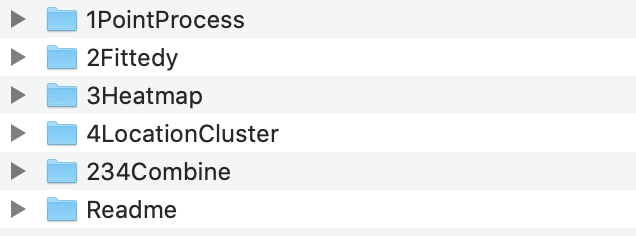
\includegraphics[width=3.5in]{name.png}
\end{center}
	\end{figure}
	\begin{enumerate}
		\item 1PointProcess
		\item 2Fittedy
		\item 3Heatmap
		\item 4LocationCluster
		\item 234Combine
		\item Readme
	\end{enumerate}
\item The preceding 5 files: 1PointProcess, 2Fittedy, 3Heatmap, 4LocationCluster, 234Combine have  the Matlab codes for creating the plots.
\item And the plot created are stored in the folder plot.
\item The Readme folder introduce the plotting process.

\end{itemize}
		\pagebreak
\section{1PointProcess}
\begin{itemize}
	\item The file PointProcess.m is the code that plots the temporal point process diagram and the corresponding congestion intensity function.
	\item The input data is: 2015\_N1\_N\_2571.mat.
	\item There are 4 output plots-- the temporal point process diagram for weekday, the temporal point process diagram for holiday, the intensity function for weekday, and the temporal point process diagram for holiday.
\end{itemize}
\begin{figure}[h!]
\begin{center}
	\vspace{-0.3in}
	\subfloat[pointprocess\_Weekday.png]{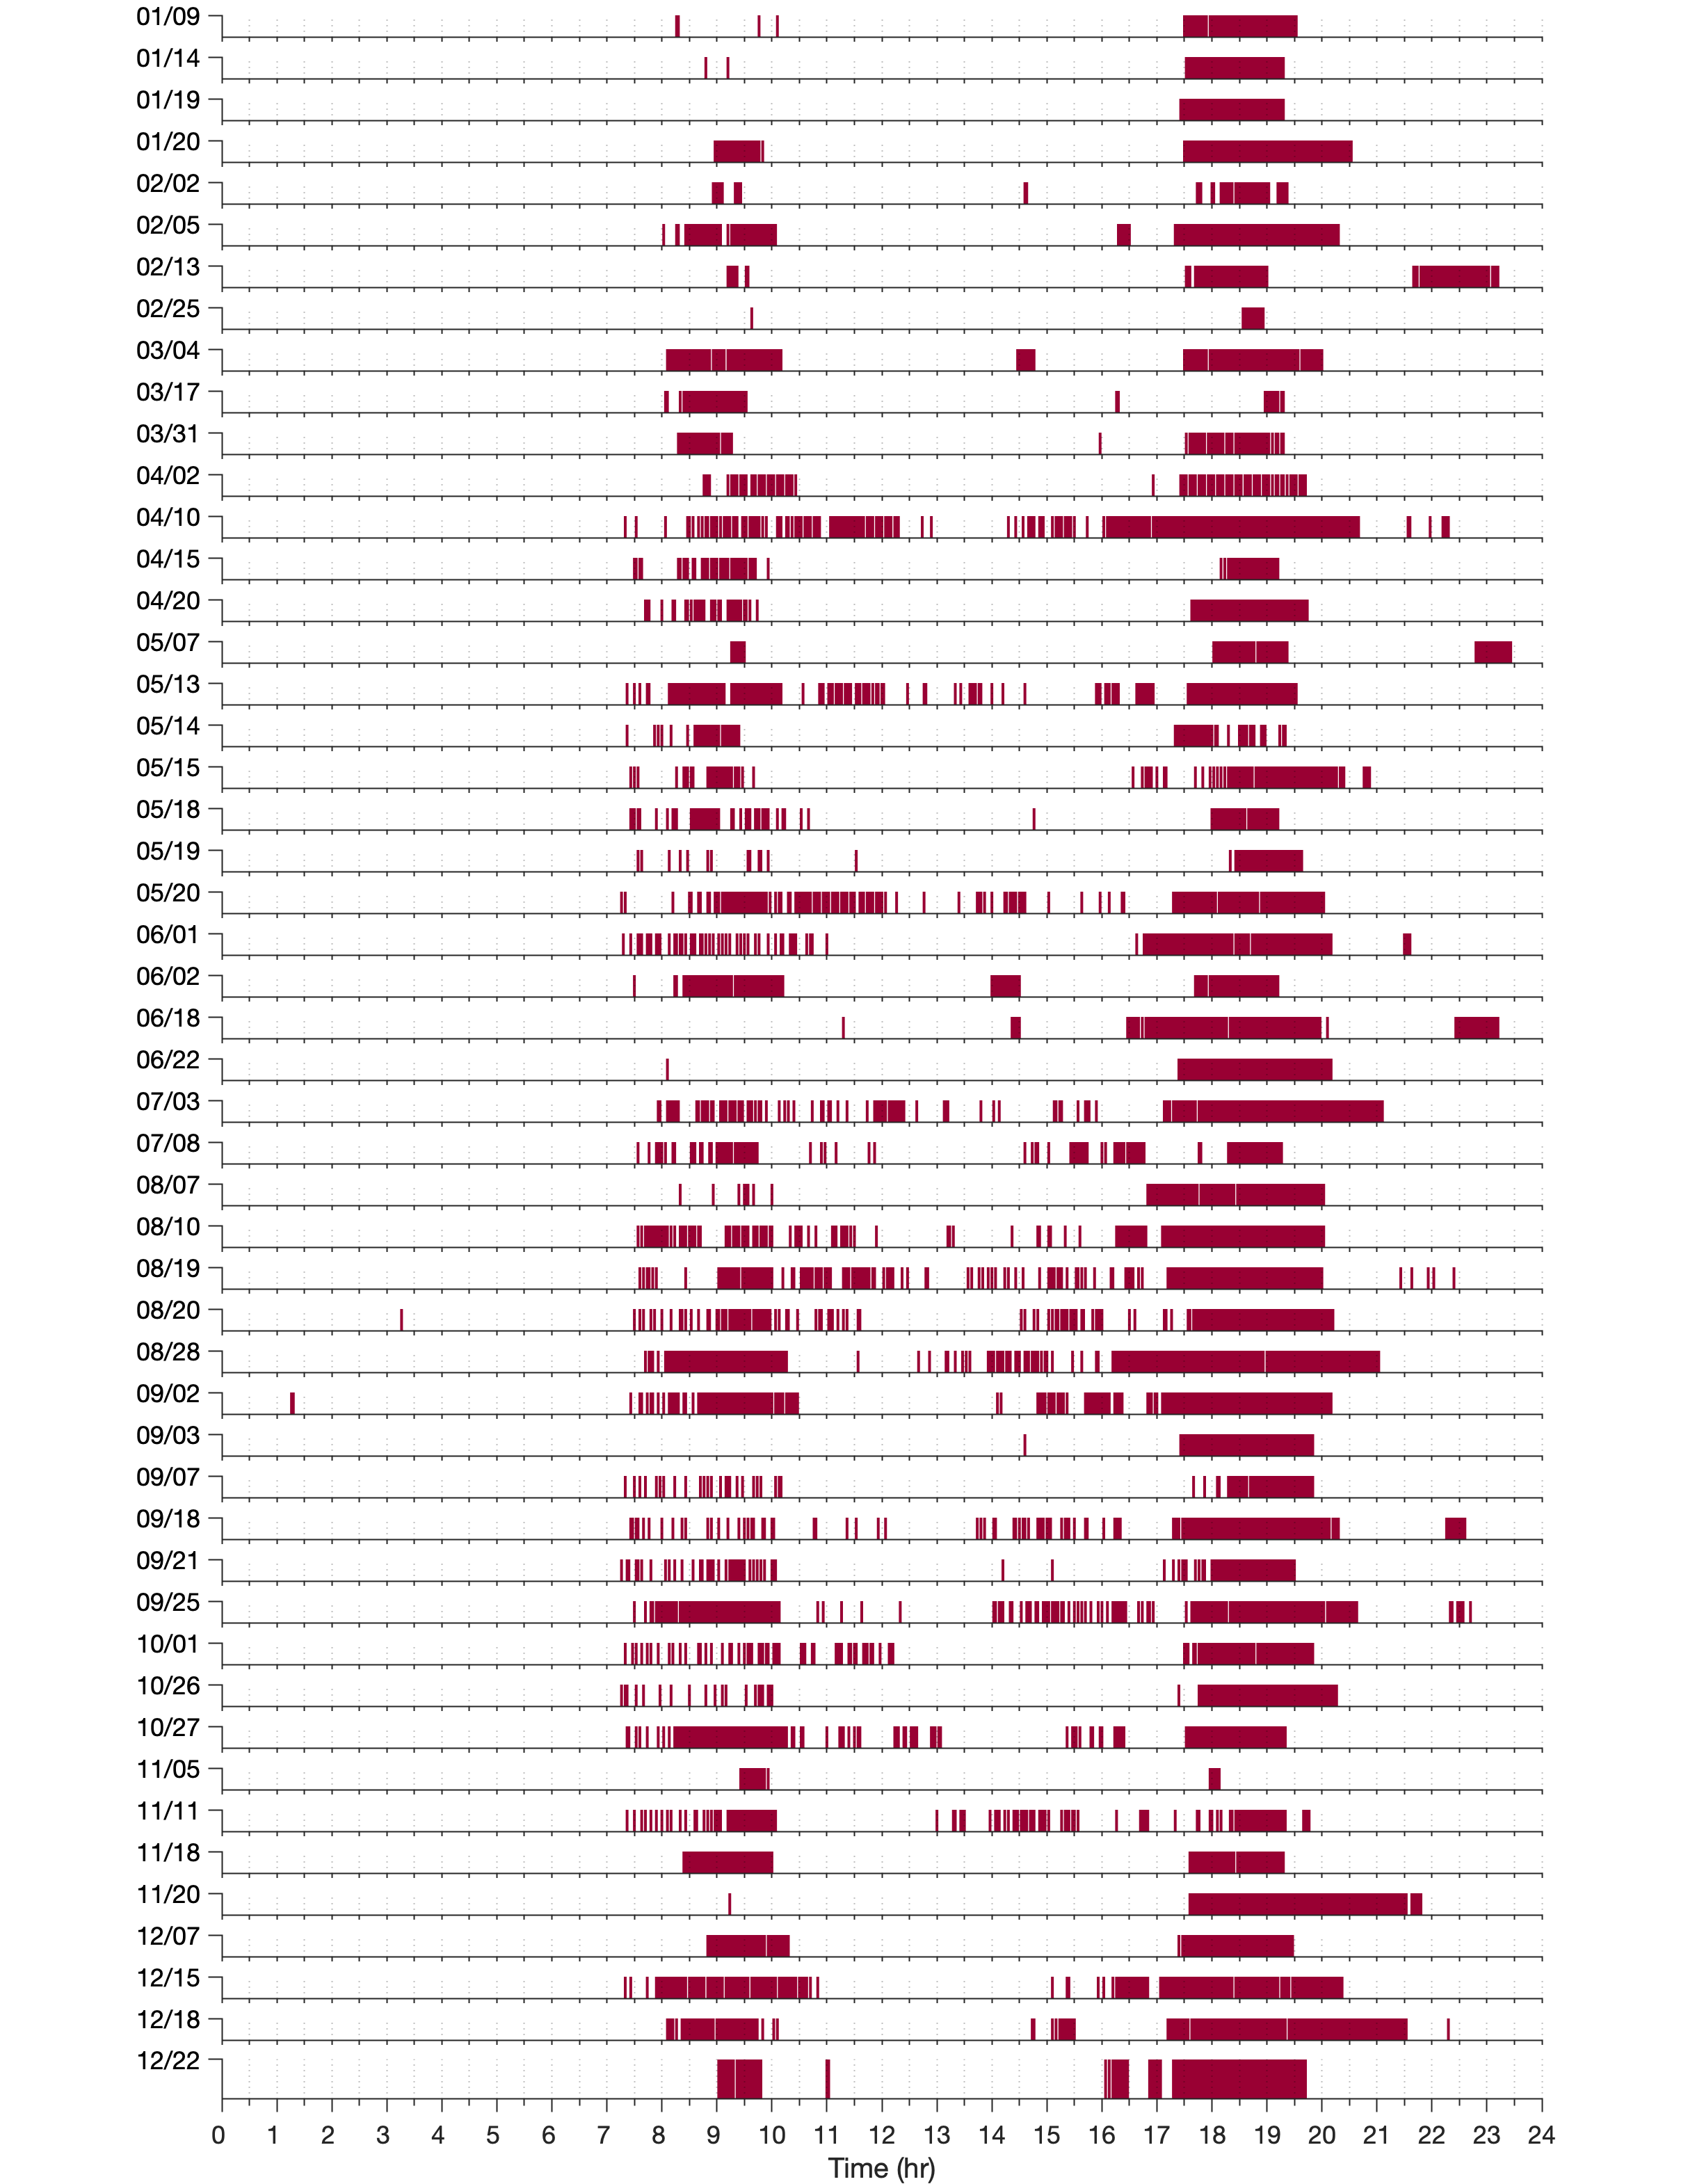
\includegraphics[width=7cm]{../1PointProcess/plot/pointprocess_Weekday.png}} 
	\subfloat[pointprocess\_Holiday.png]{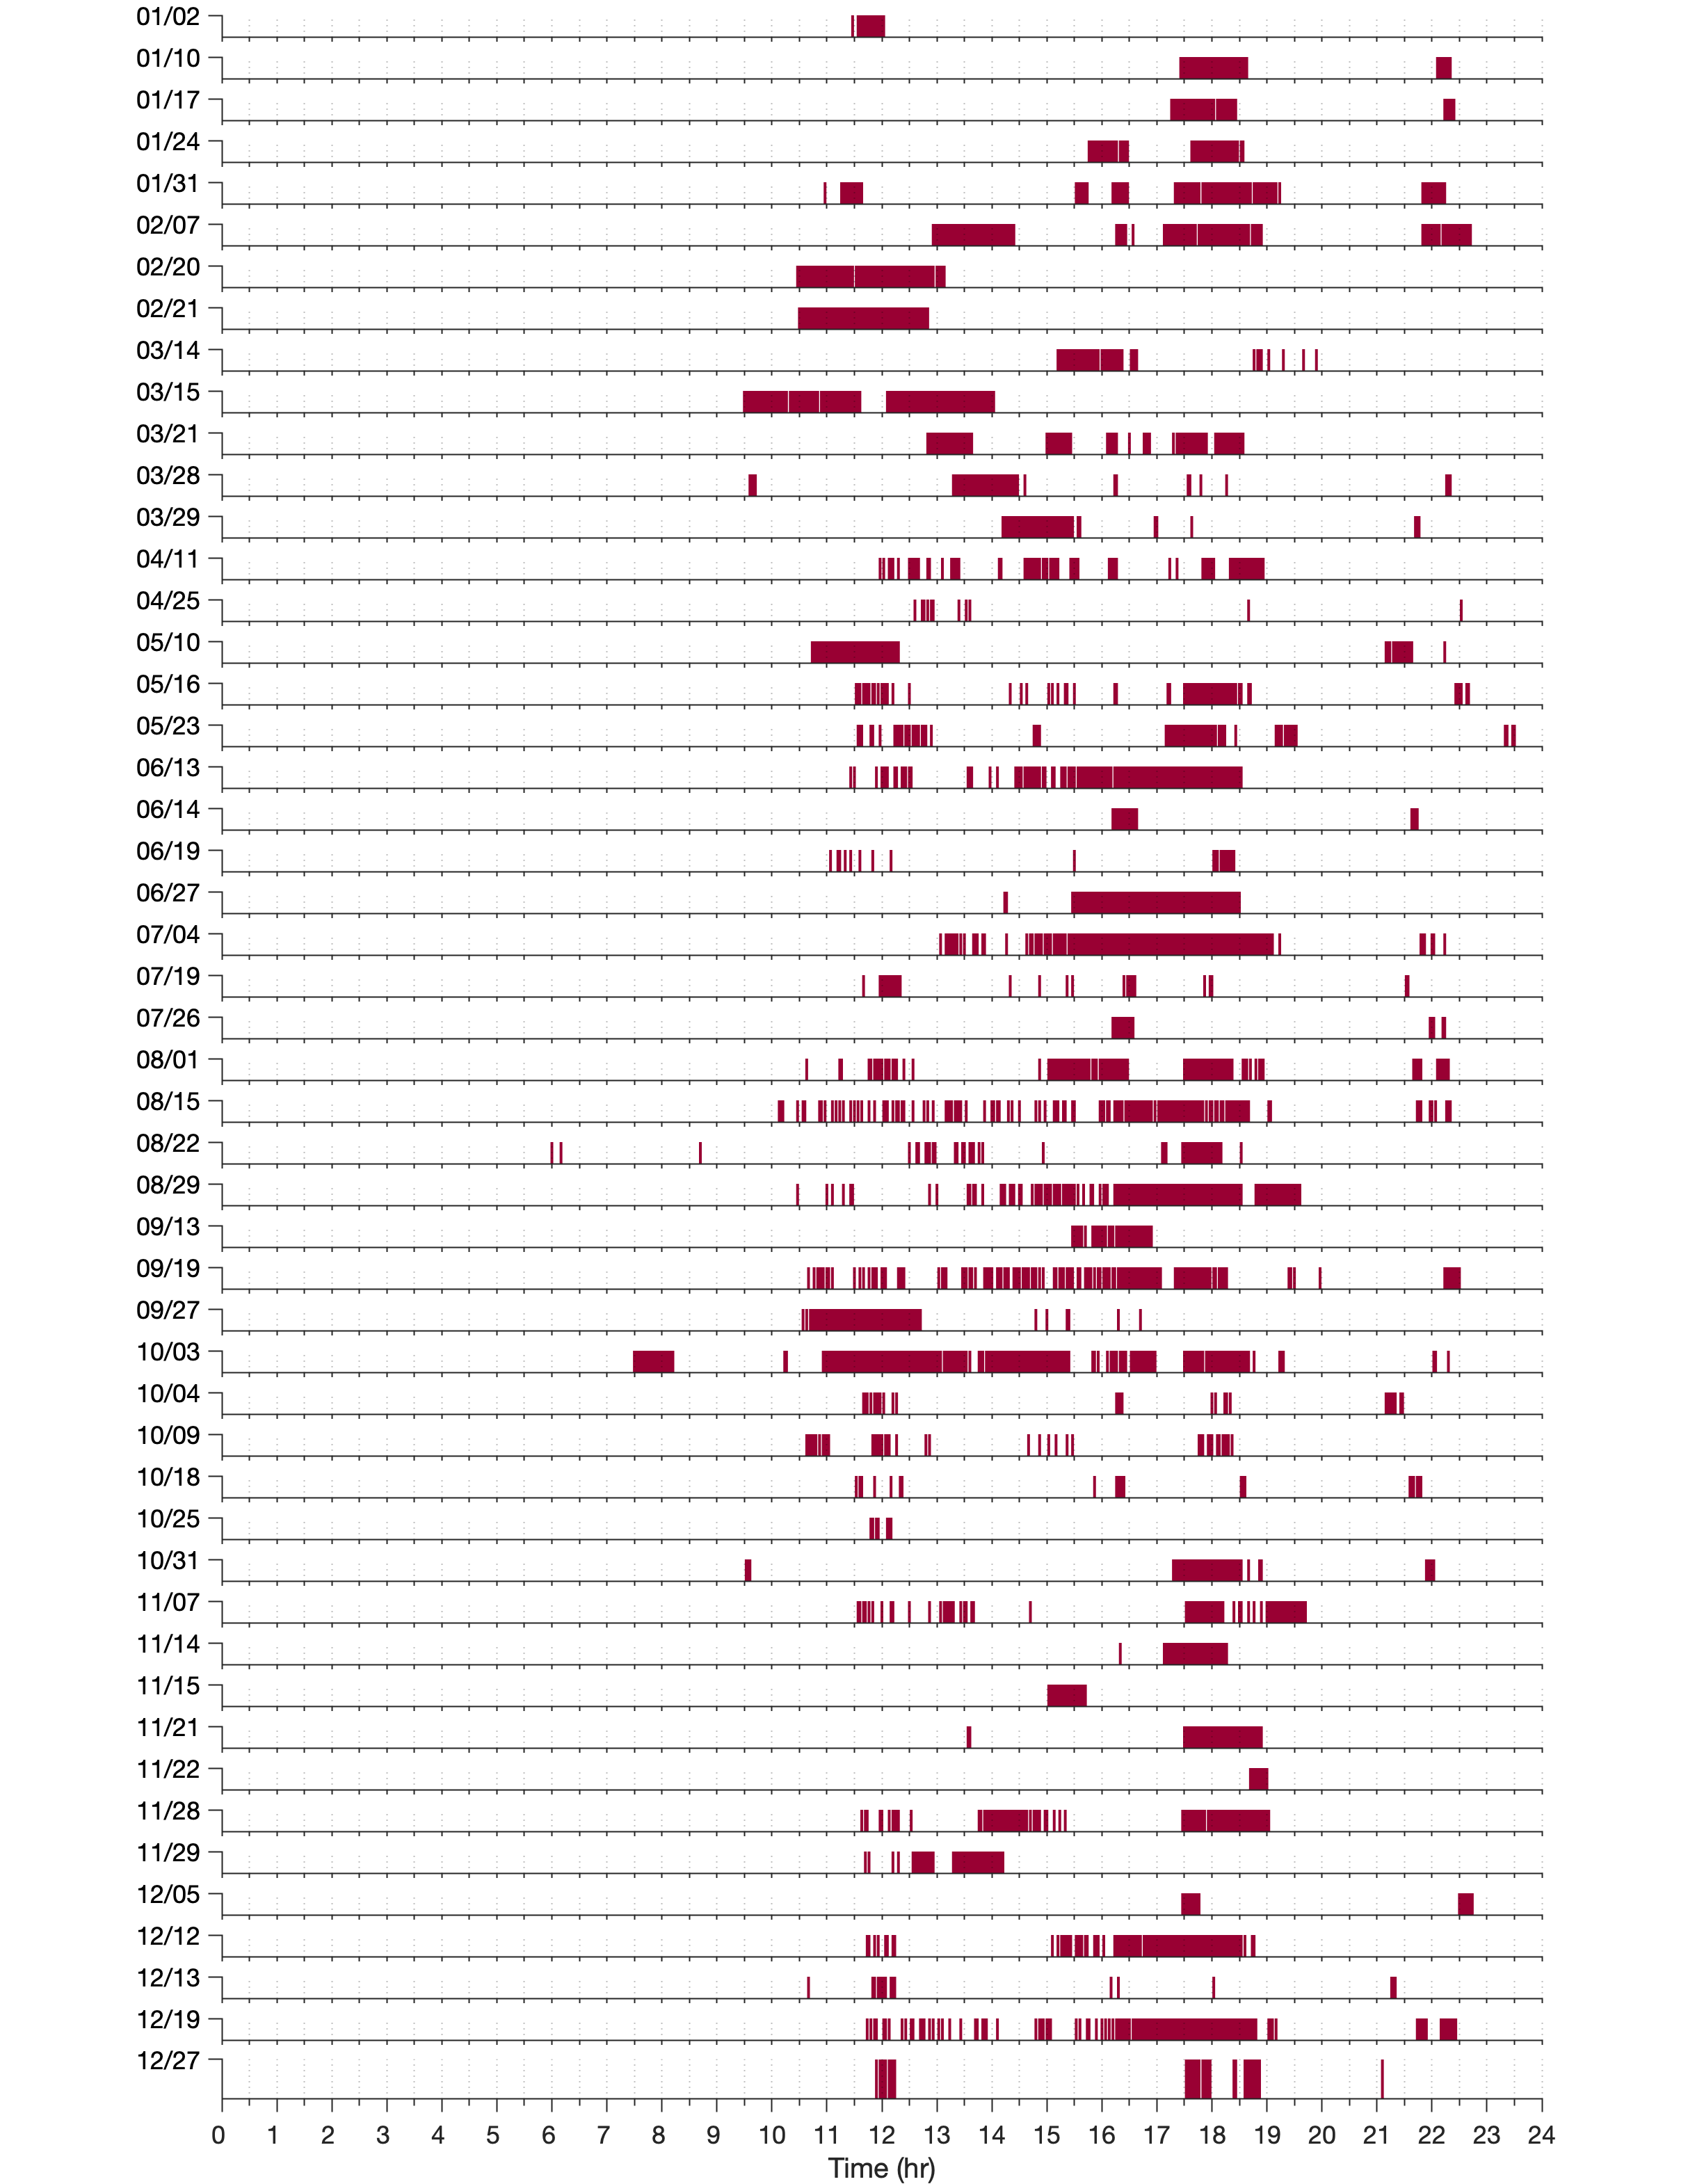
\includegraphics[width=7cm]{../1PointProcess/plot/pointprocess_Holiday.png}}
	\caption{Point Process Diagram}%
\end{center}
\end{figure}


\begin{figure}[h!]
\begin{center}
		\subfloat[intensity\_Weekday.png]{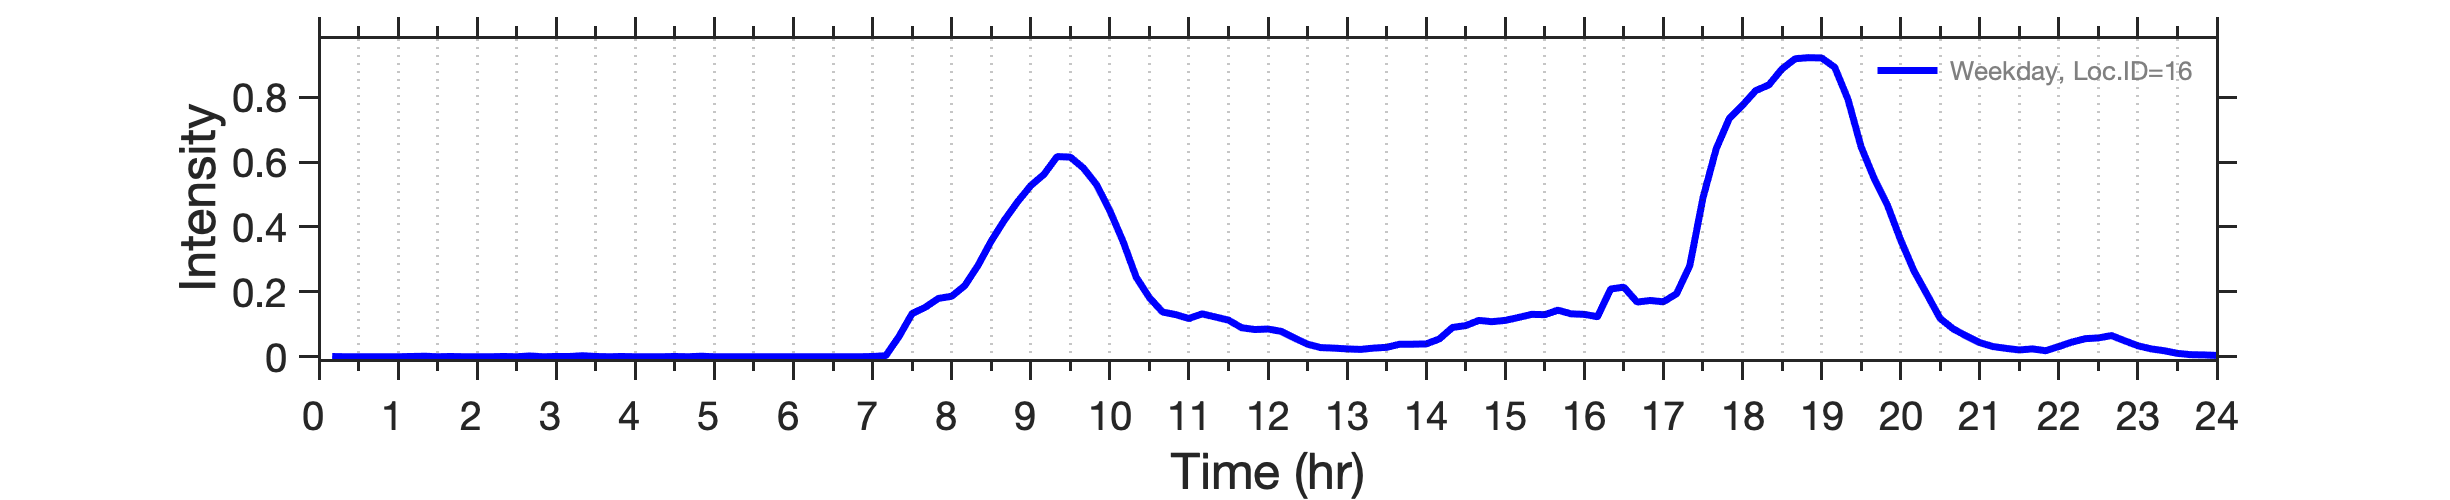
\includegraphics[width=7cm]{../1PointProcess/plot/intensity_Weekday.png}} 
	\subfloat[intensity\_Holiday.png]{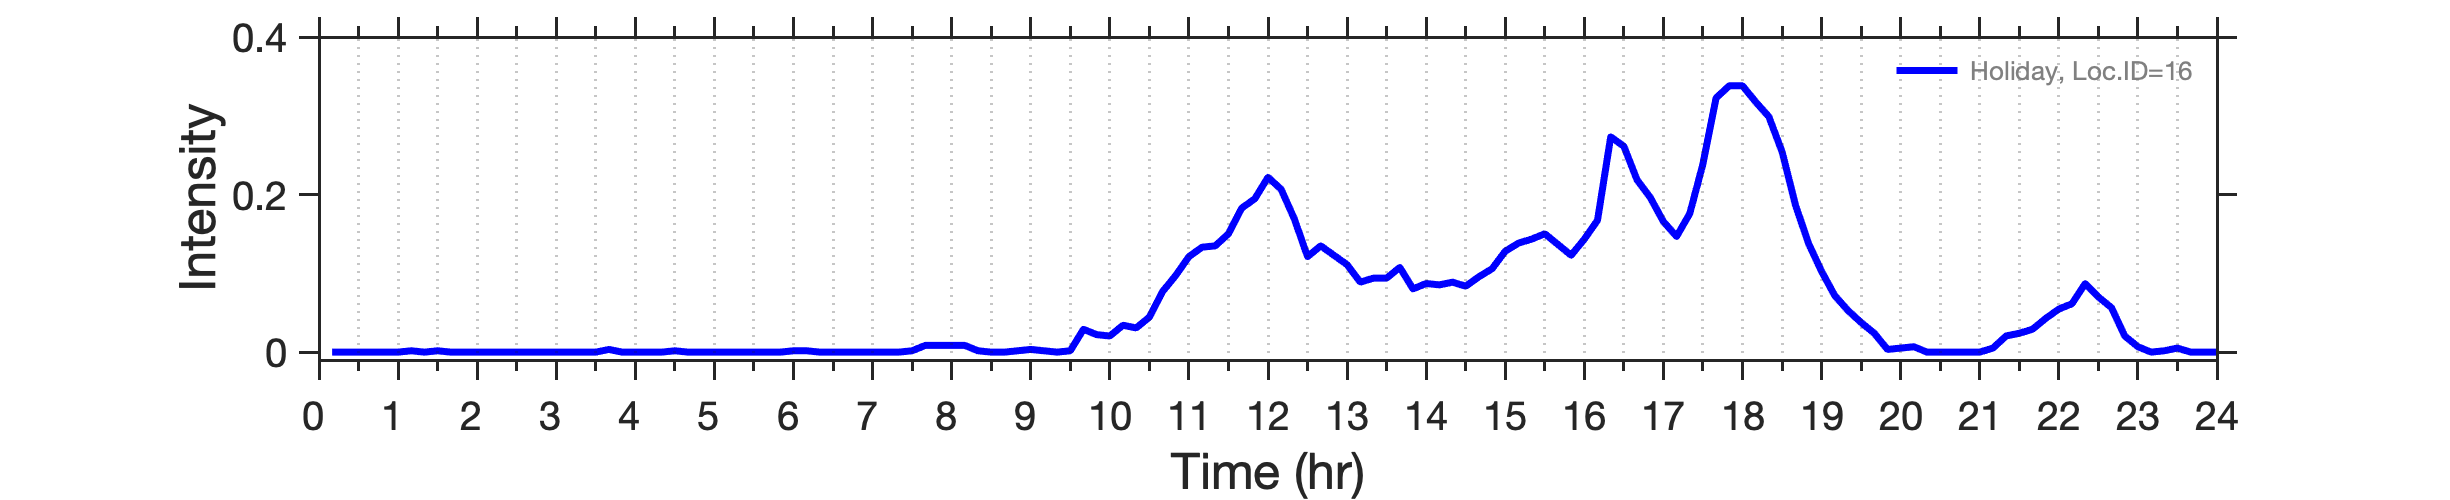
\includegraphics[width=7cm]{../1PointProcess/plot/intensity_Holiday.png}}
	\caption{Intensity function}%
\end{center}
\end{figure}





\section{2Fittedy}
\begin{itemize}
	\item The file Fittedy.m this file is the code that plots the results from KCFC
	\item The KCFC results are stored in the file  detail\_weekday\_7.mat (with number of clusters $K_1=7$) and	detail\_holiday\_5.mat (with number of clusters $K_2=5$).
\end{itemize}


\begin{figure}[h!]

	\begin{center}
			\begin{tabular}{cccc}
			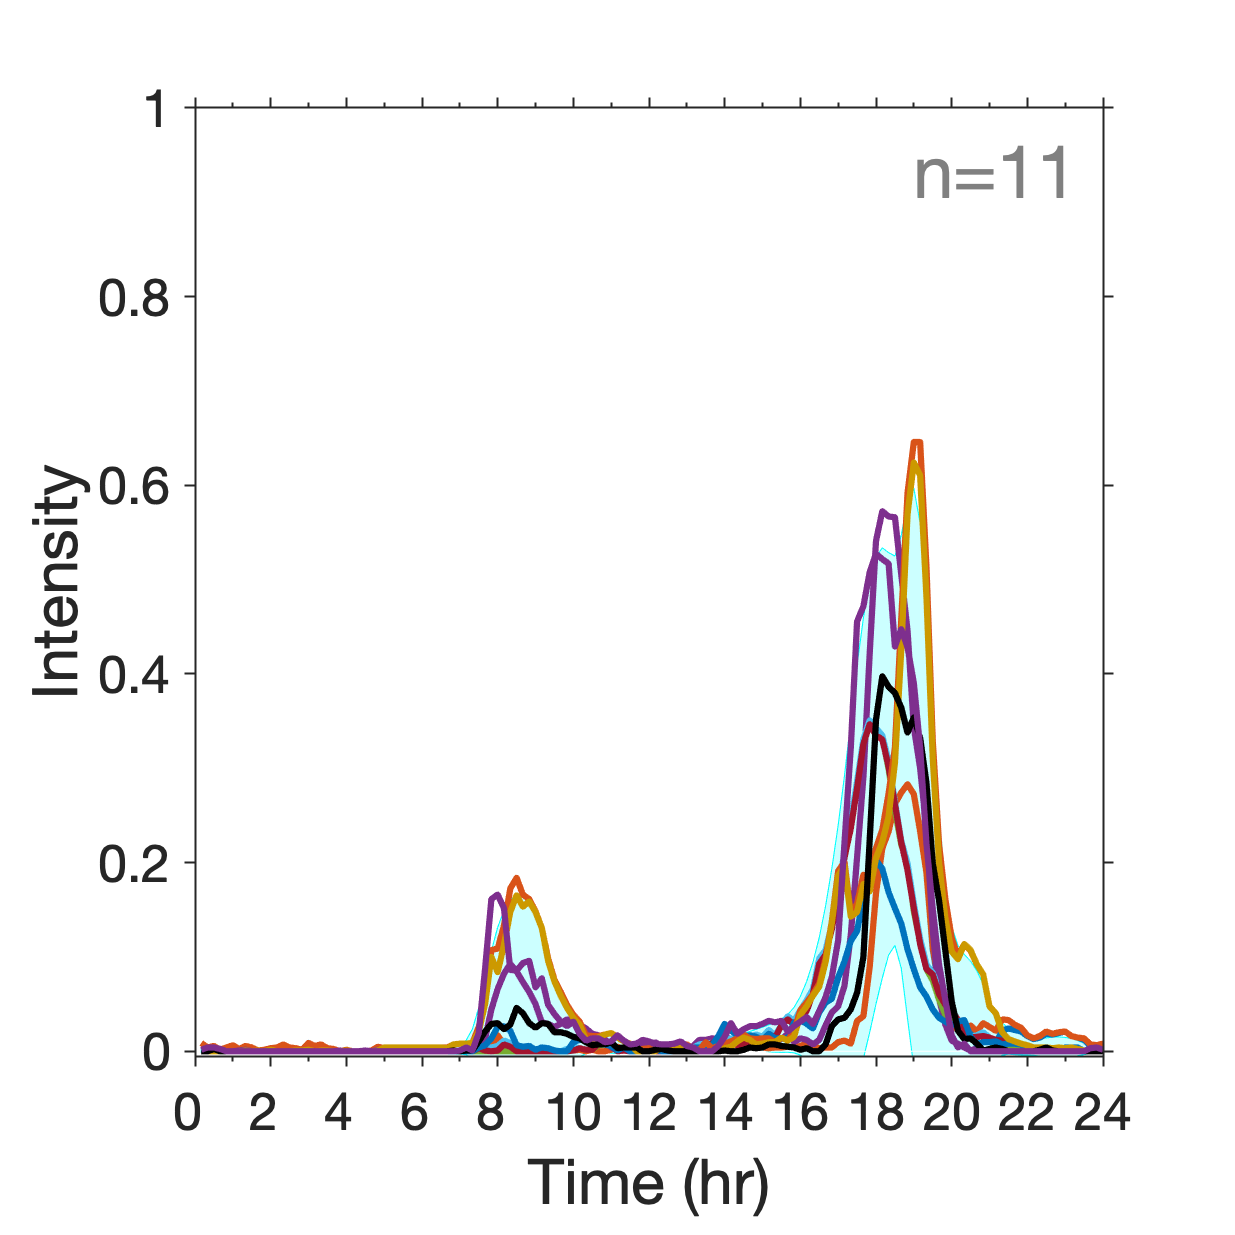
\includegraphics[scale=0.1]{../2Fittedy/plot/weekday_7/fitted_y_cluster7_1.eps} 
			&\hspace*{-0.6cm}
			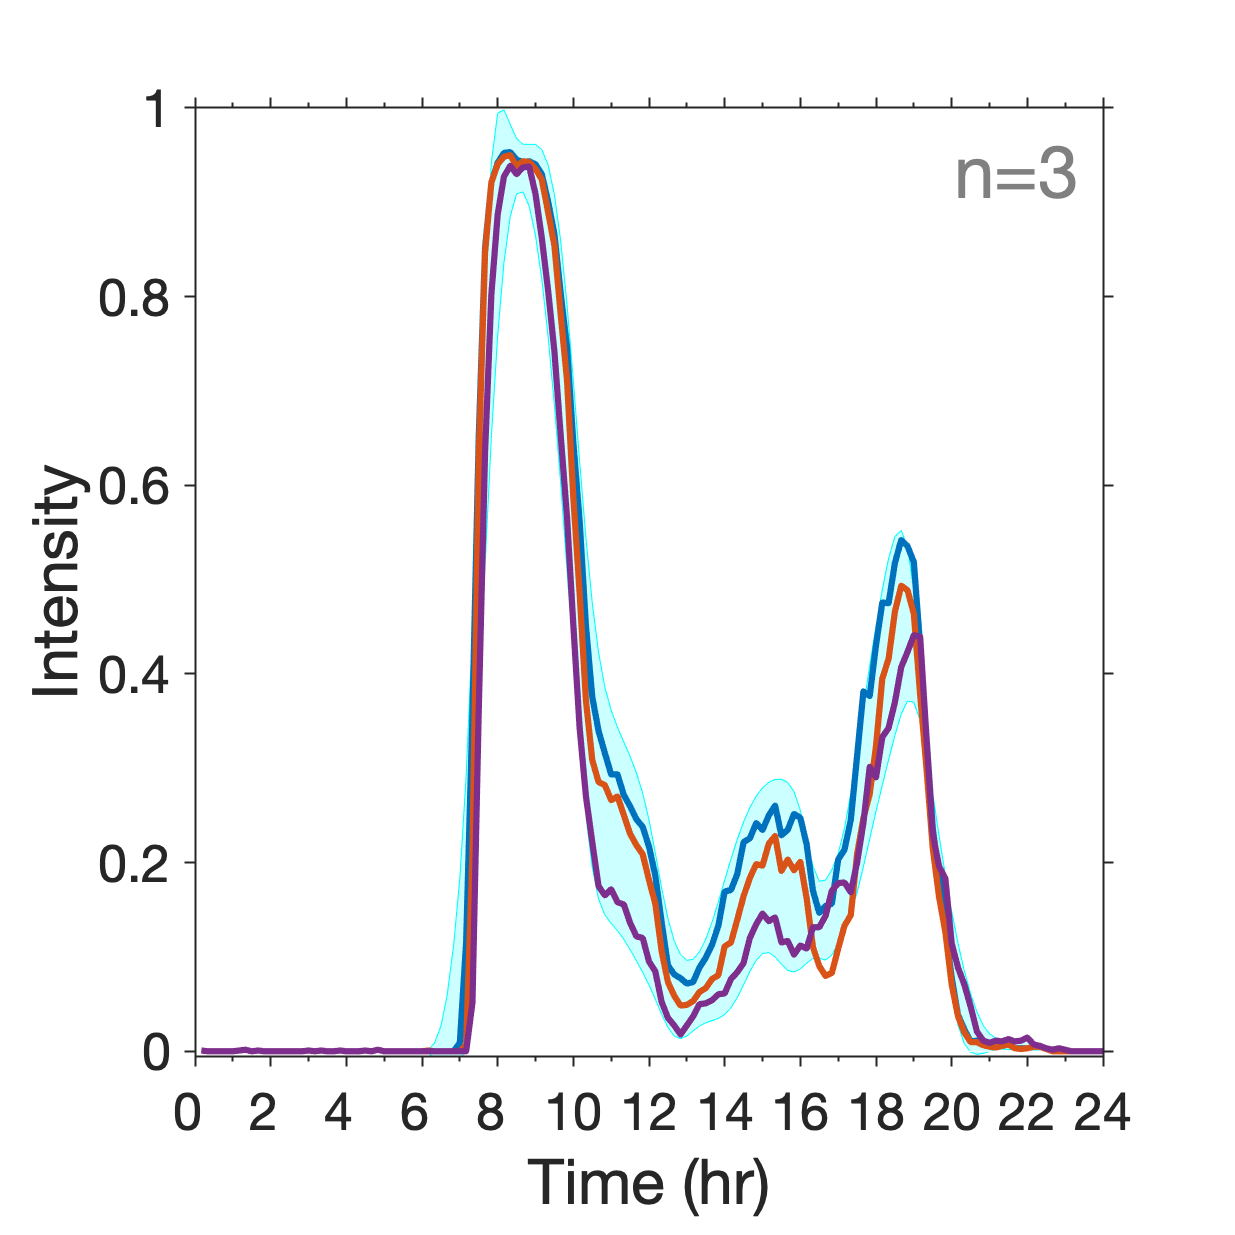
\includegraphics[scale=0.1]{../2Fittedy/plot/weekday_7/fitted_y_cluster7_2.eps} 
			&\hspace*{-0.6cm}
			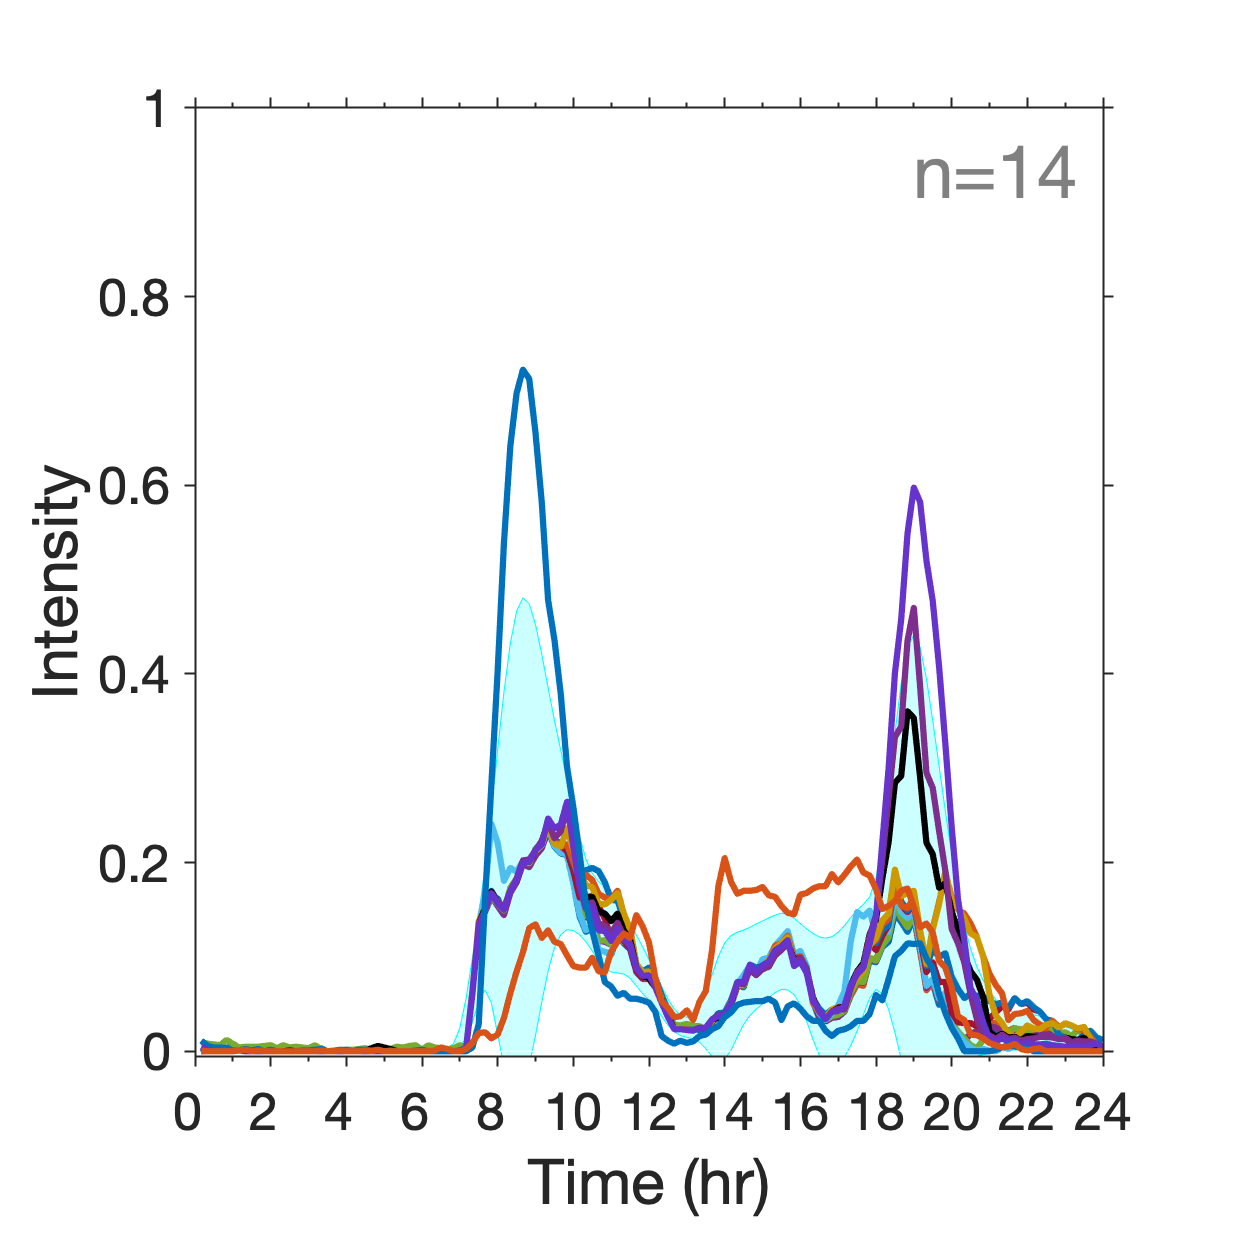
\includegraphics[scale=0.1]{../2Fittedy/plot/weekday_7/fitted_y_cluster7_3.eps} 
			&\hspace*{-0.6cm}
			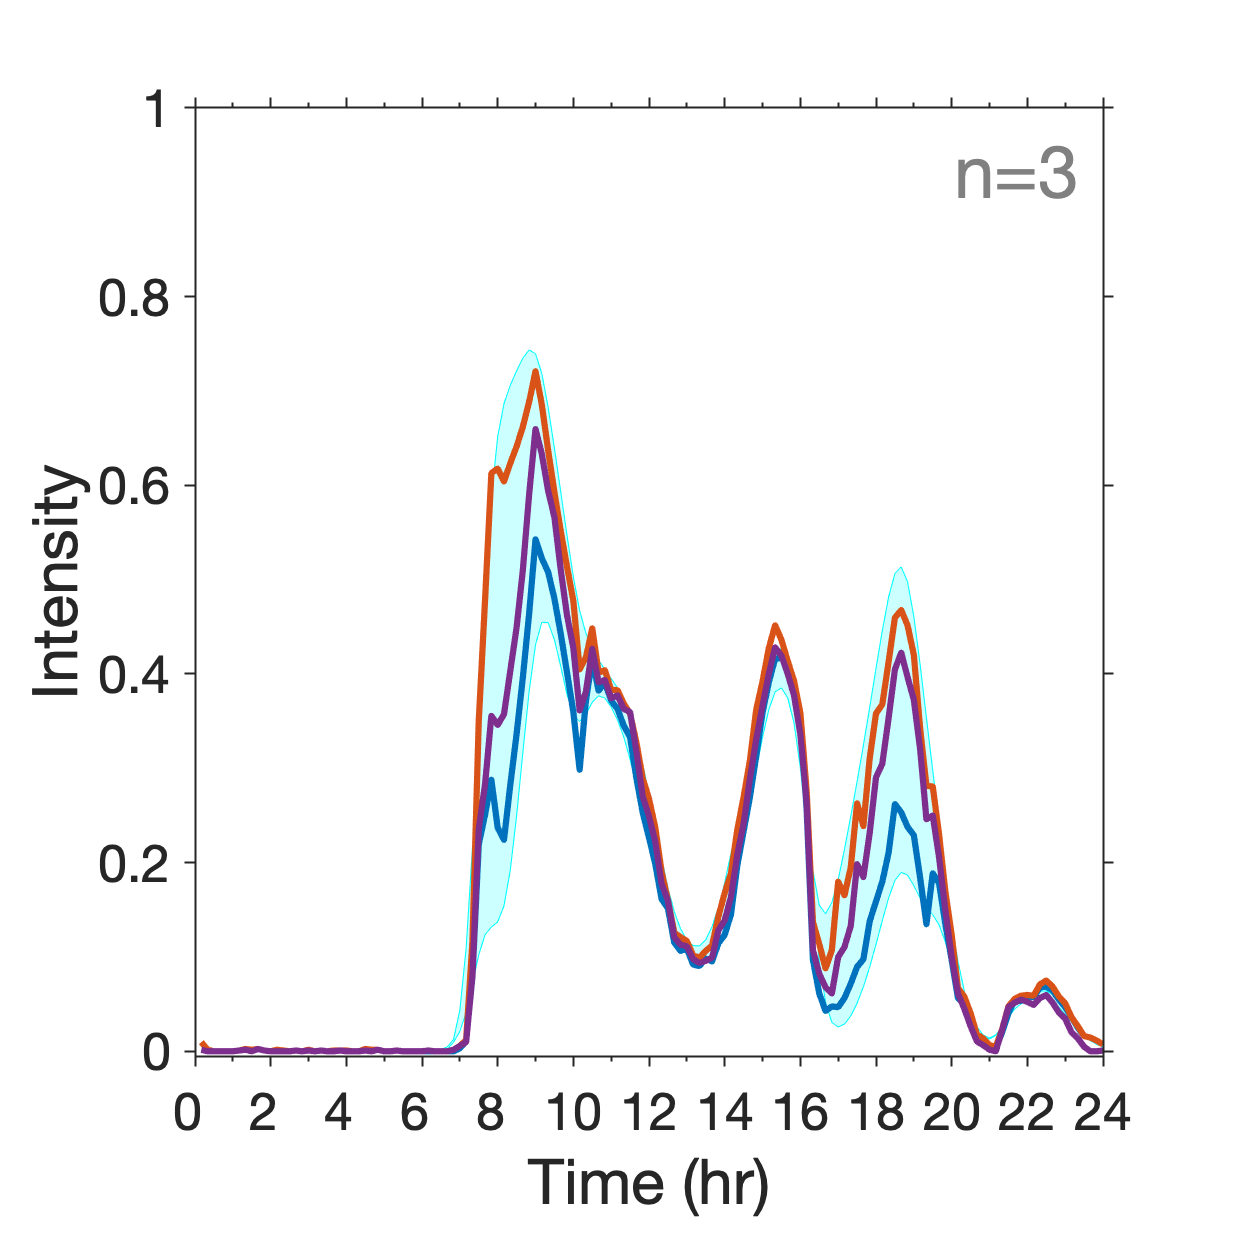
\includegraphics[scale=0.1]{../2Fittedy/plot/weekday_7/fitted_y_cluster7_4.eps} \\
			
			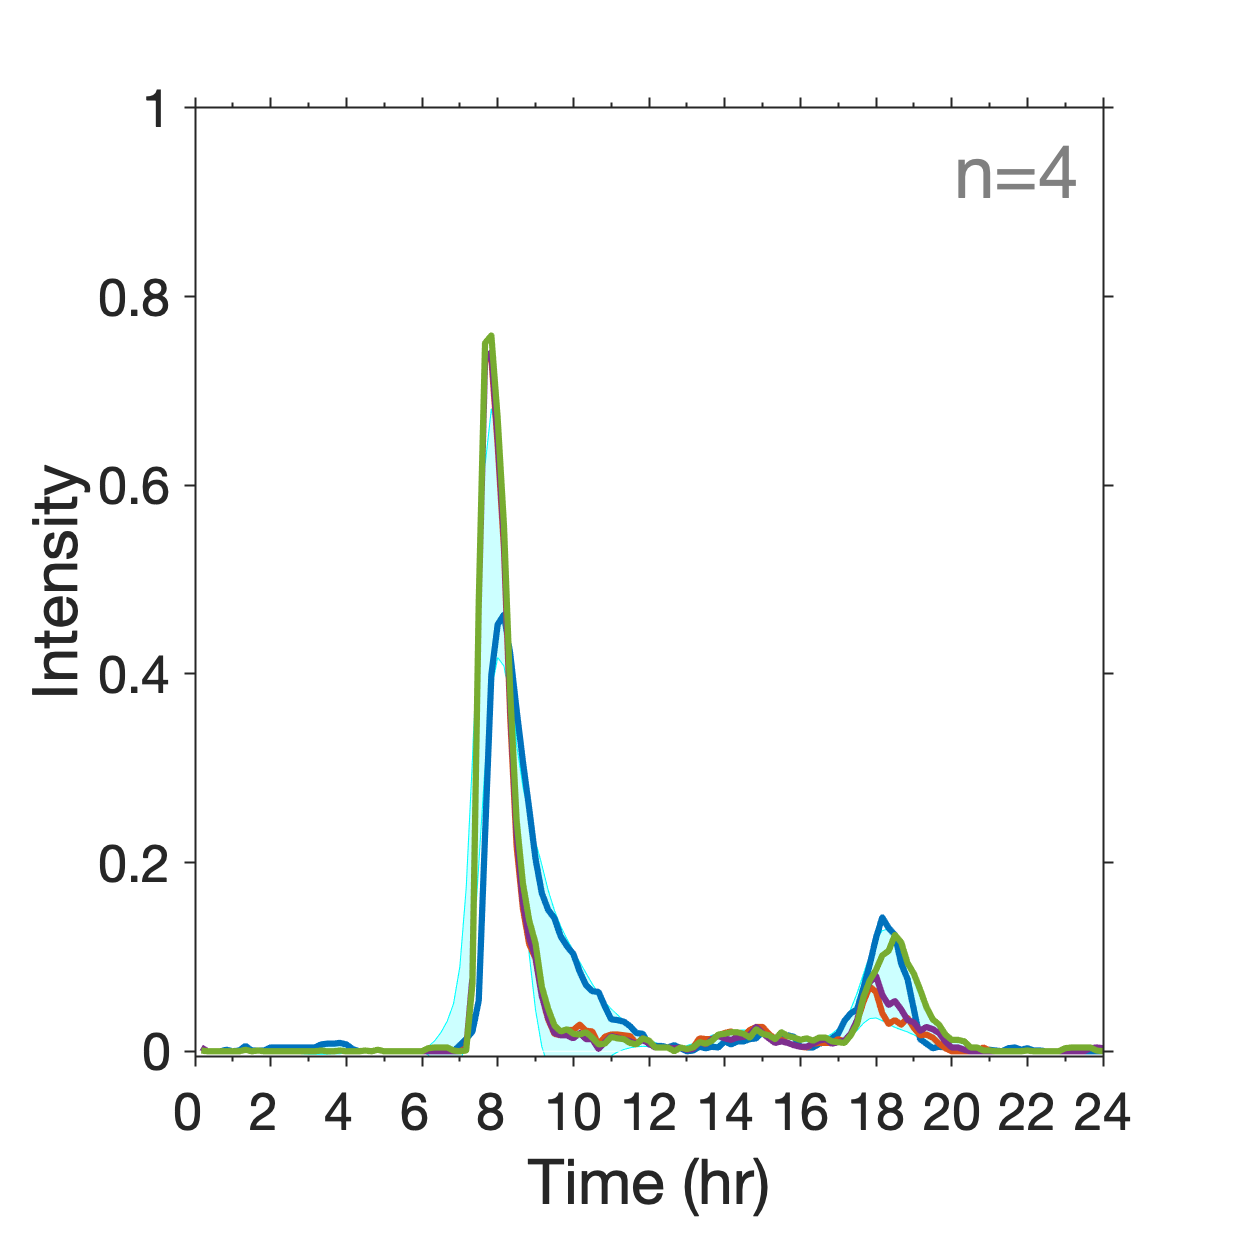
\includegraphics[scale=0.1]{../2Fittedy/plot/weekday_7/fitted_y_cluster7_5.eps} 
			&\hspace*{-0.6cm}
			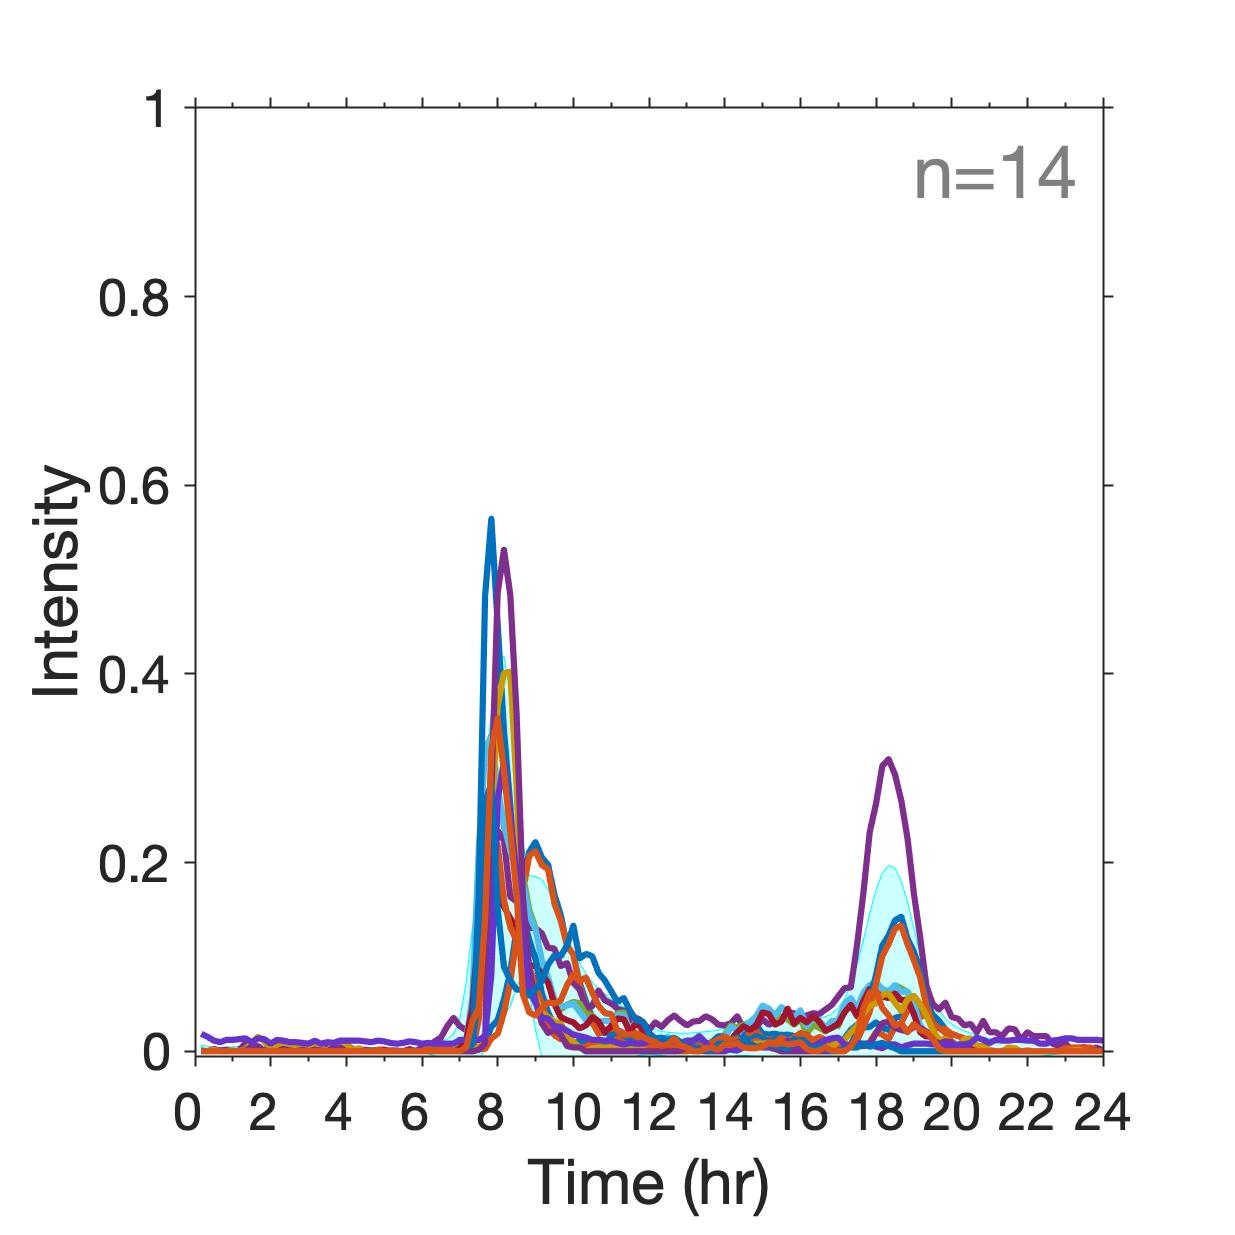
\includegraphics[scale=0.1]{../2Fittedy/plot/weekday_7/fitted_y_cluster7_6.eps} 
			&\hspace*{-0.6cm}
			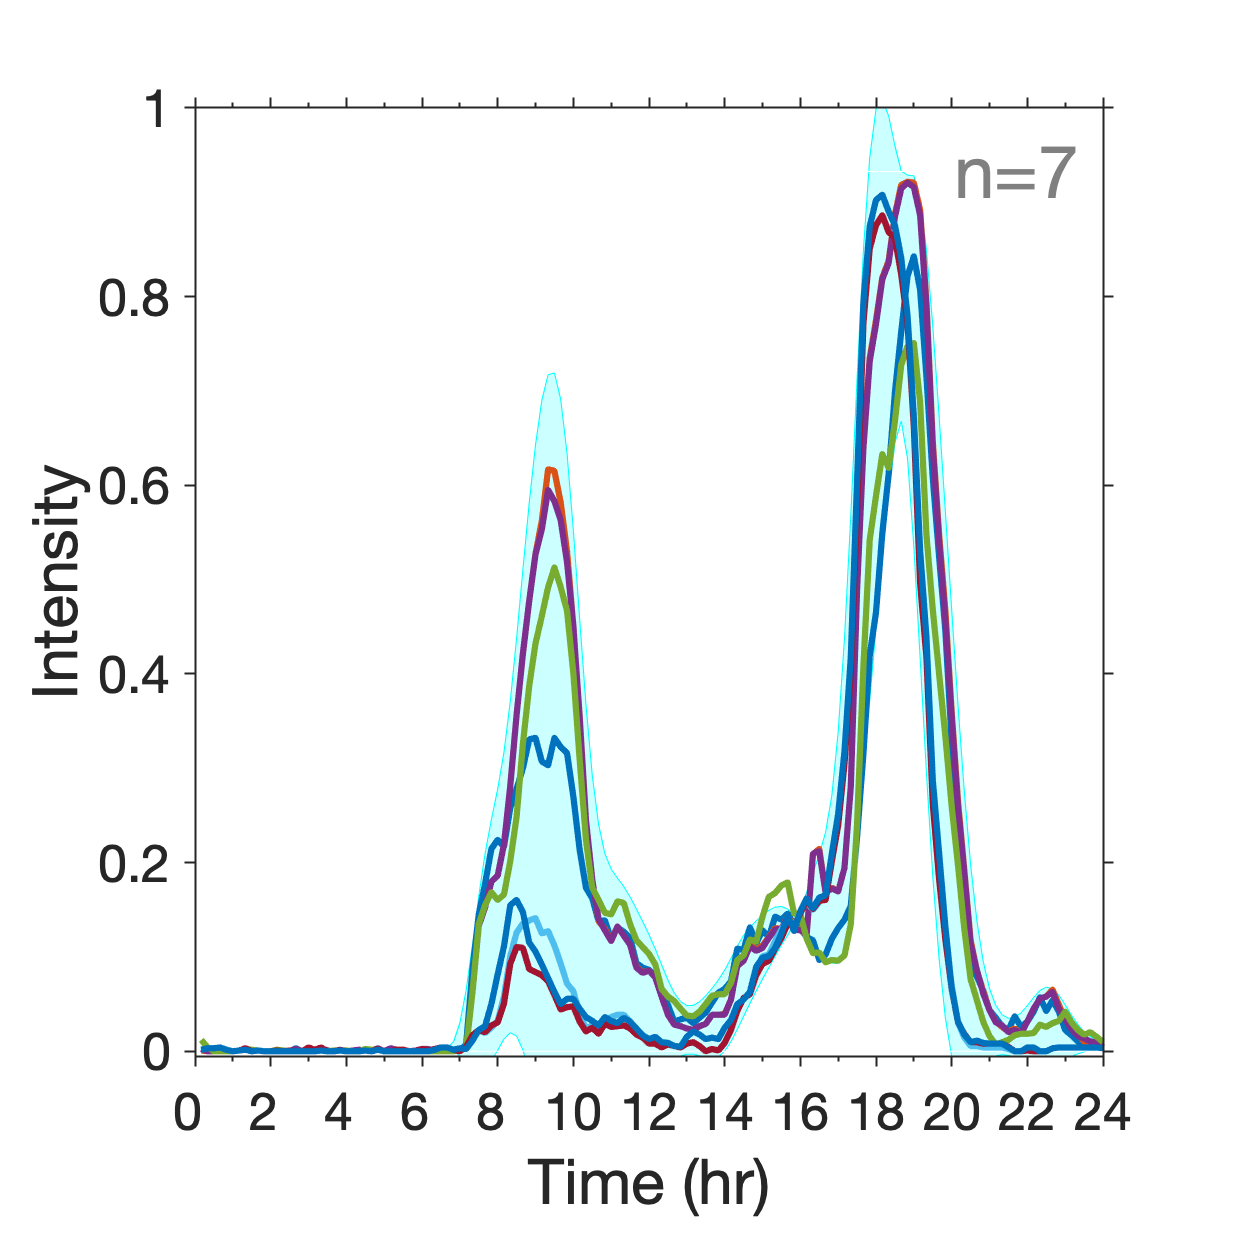
\includegraphics[scale=0.1]{../2Fittedy/plot/weekday_7/fitted_y_cluster7_7.eps}
			&\hspace*{-0.6cm}
			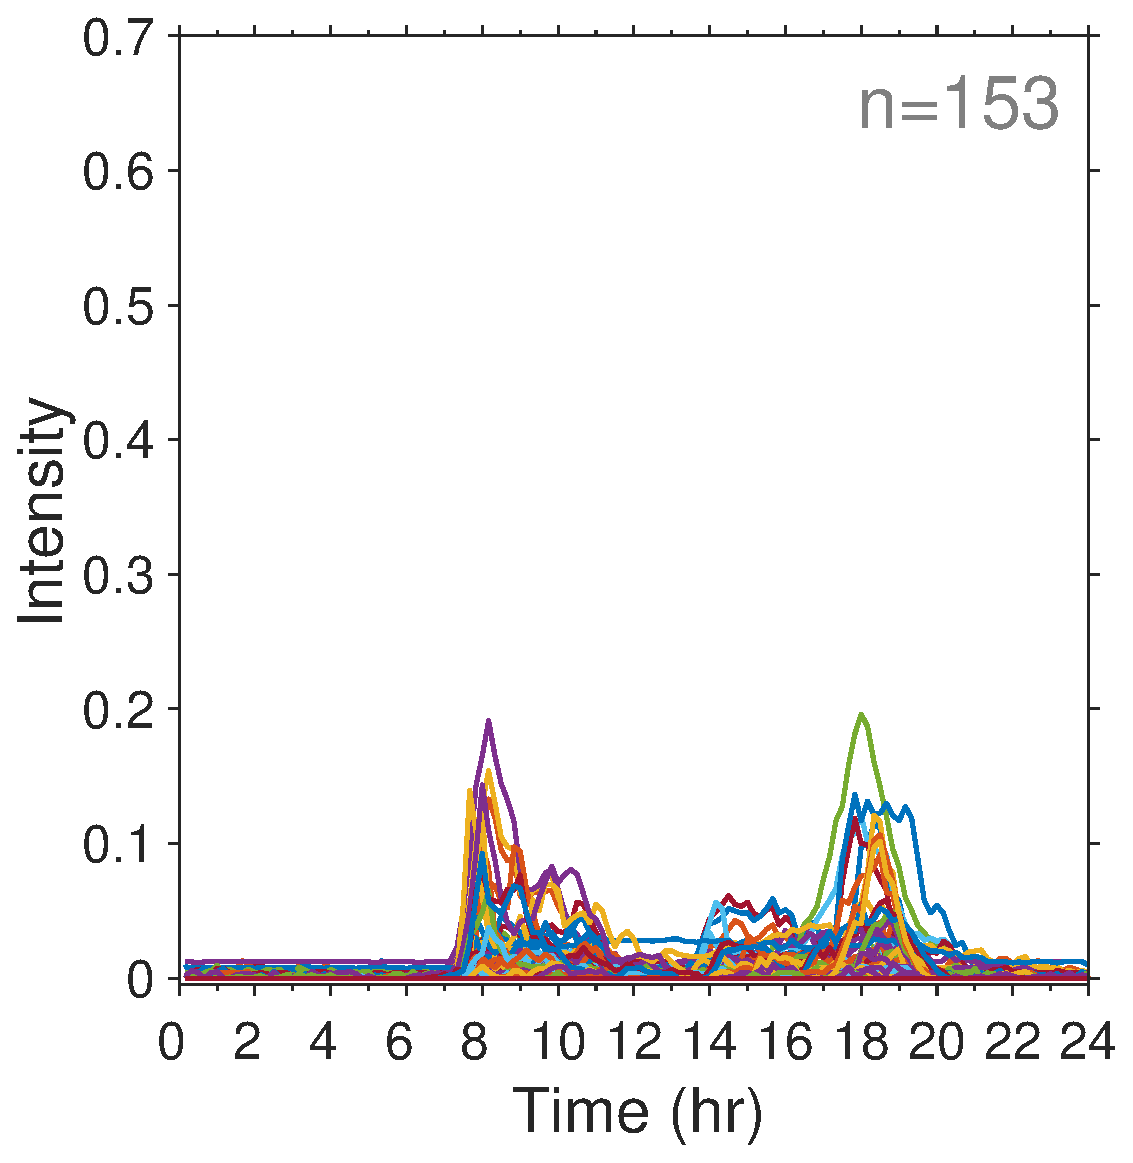
\includegraphics[scale=0.1]{../2Fittedy/plot/weekday_7/remove_data.eps}
		\end{tabular}
		
		
		\caption{Weekdays ($K_1=7$)}
		\label{Fig:clustering_Weekdays}		
	\end{center}

\end{figure}

\begin{figure}[h!]
	
	\begin{center}
		\begin{tabular}{cccc}
			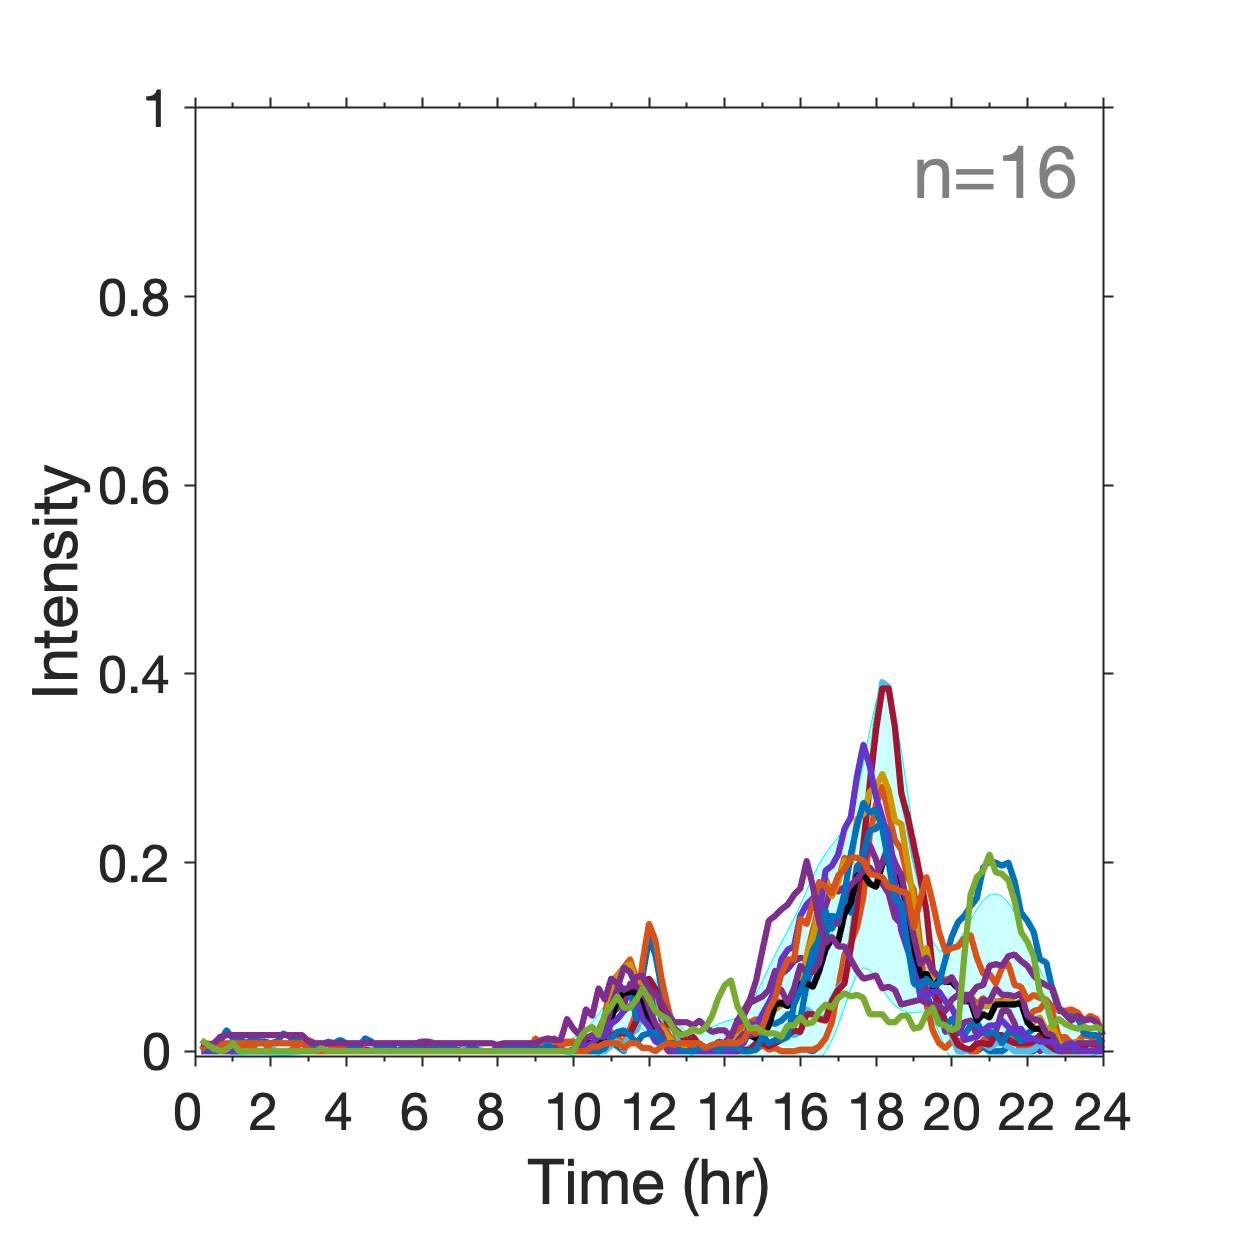
\includegraphics[scale=0.1]{../2Fittedy/plot/holiday_5/fitted_y_cluster5_1.eps} 
			&\hspace*{-0.6cm}
			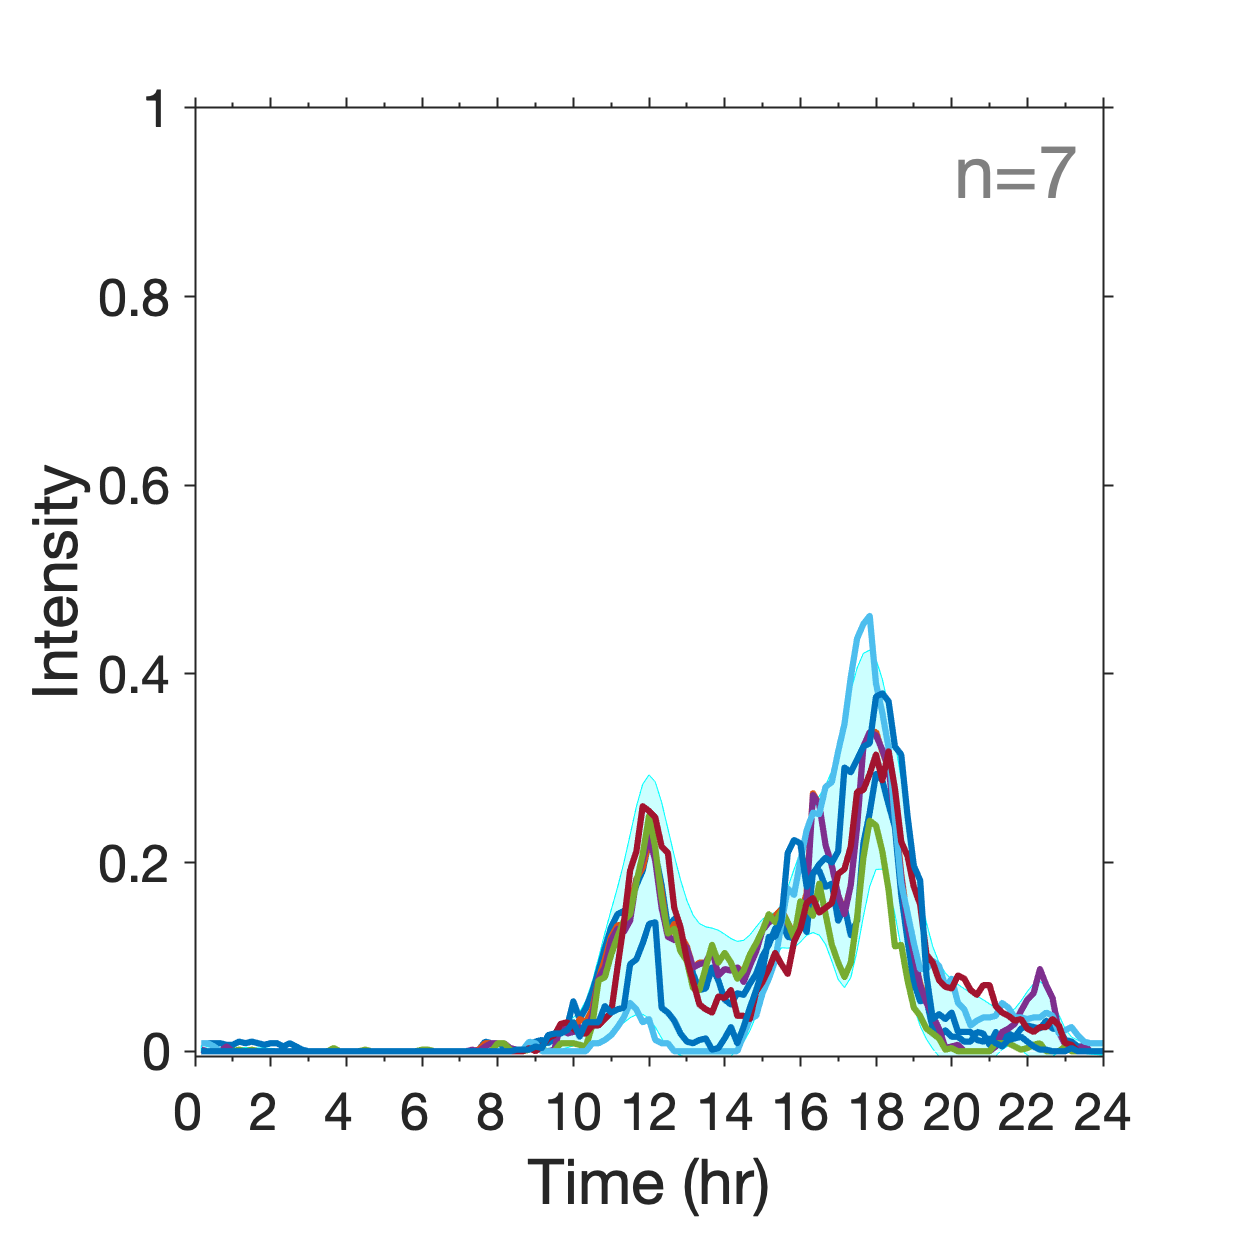
\includegraphics[scale=0.1]{../2Fittedy/plot/holiday_5/fitted_y_cluster5_2.eps} 
			&\hspace*{-0.6cm}
			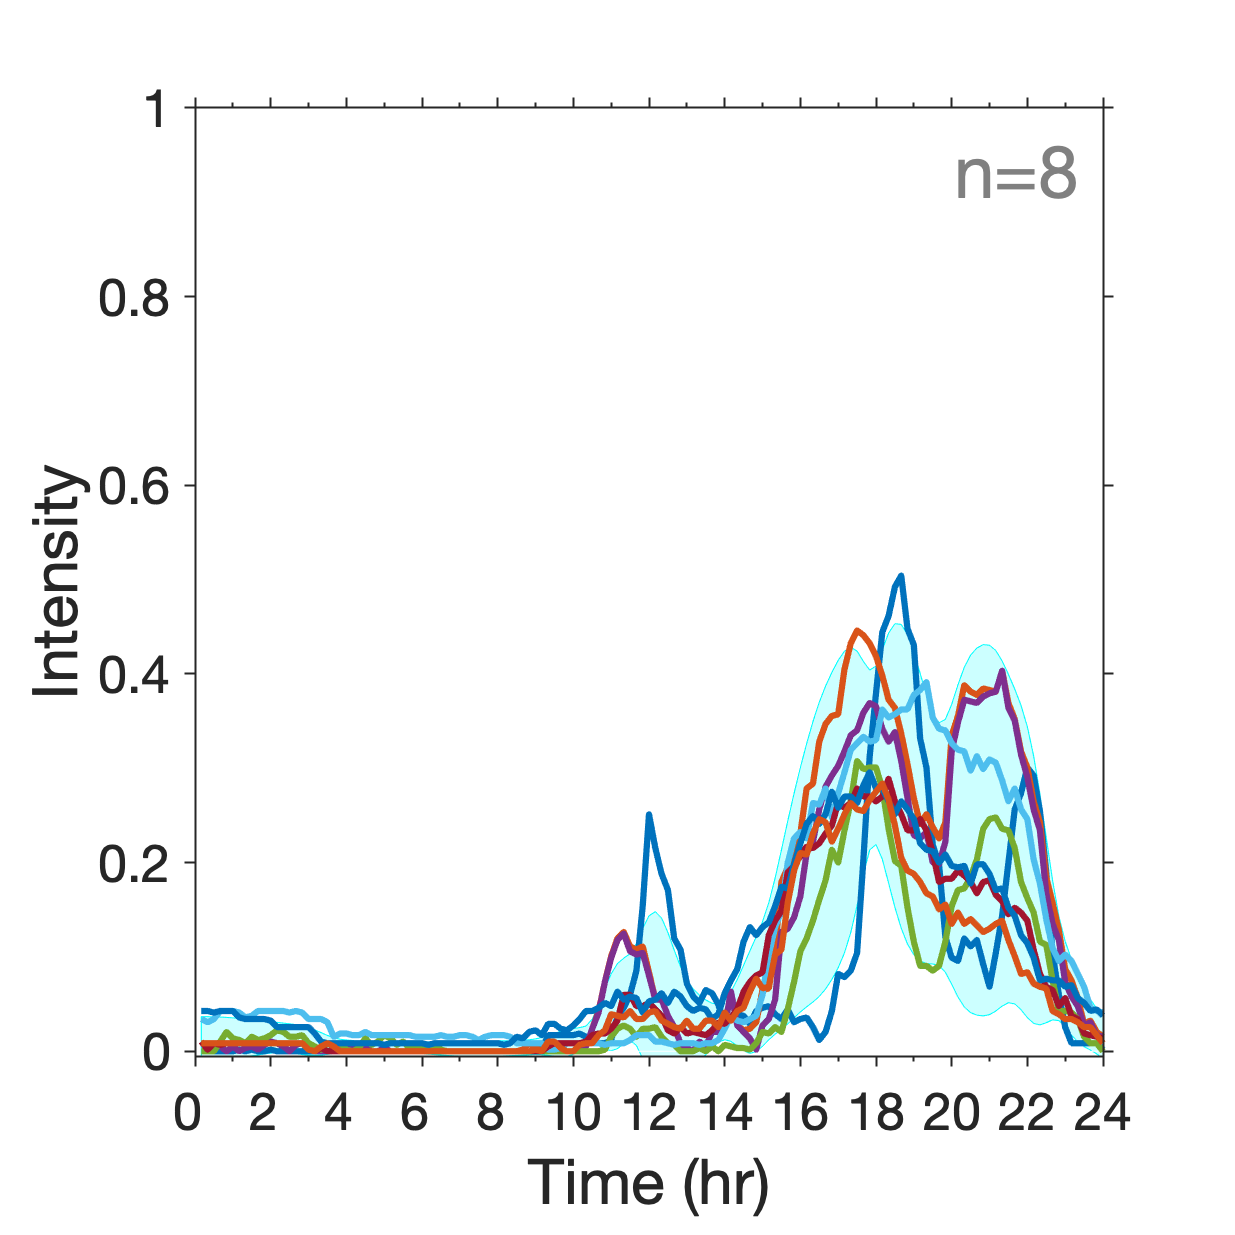
\includegraphics[scale=0.1]{../2Fittedy/plot/holiday_5/fitted_y_cluster5_3.eps} 
			&\hspace*{-0.6cm}
			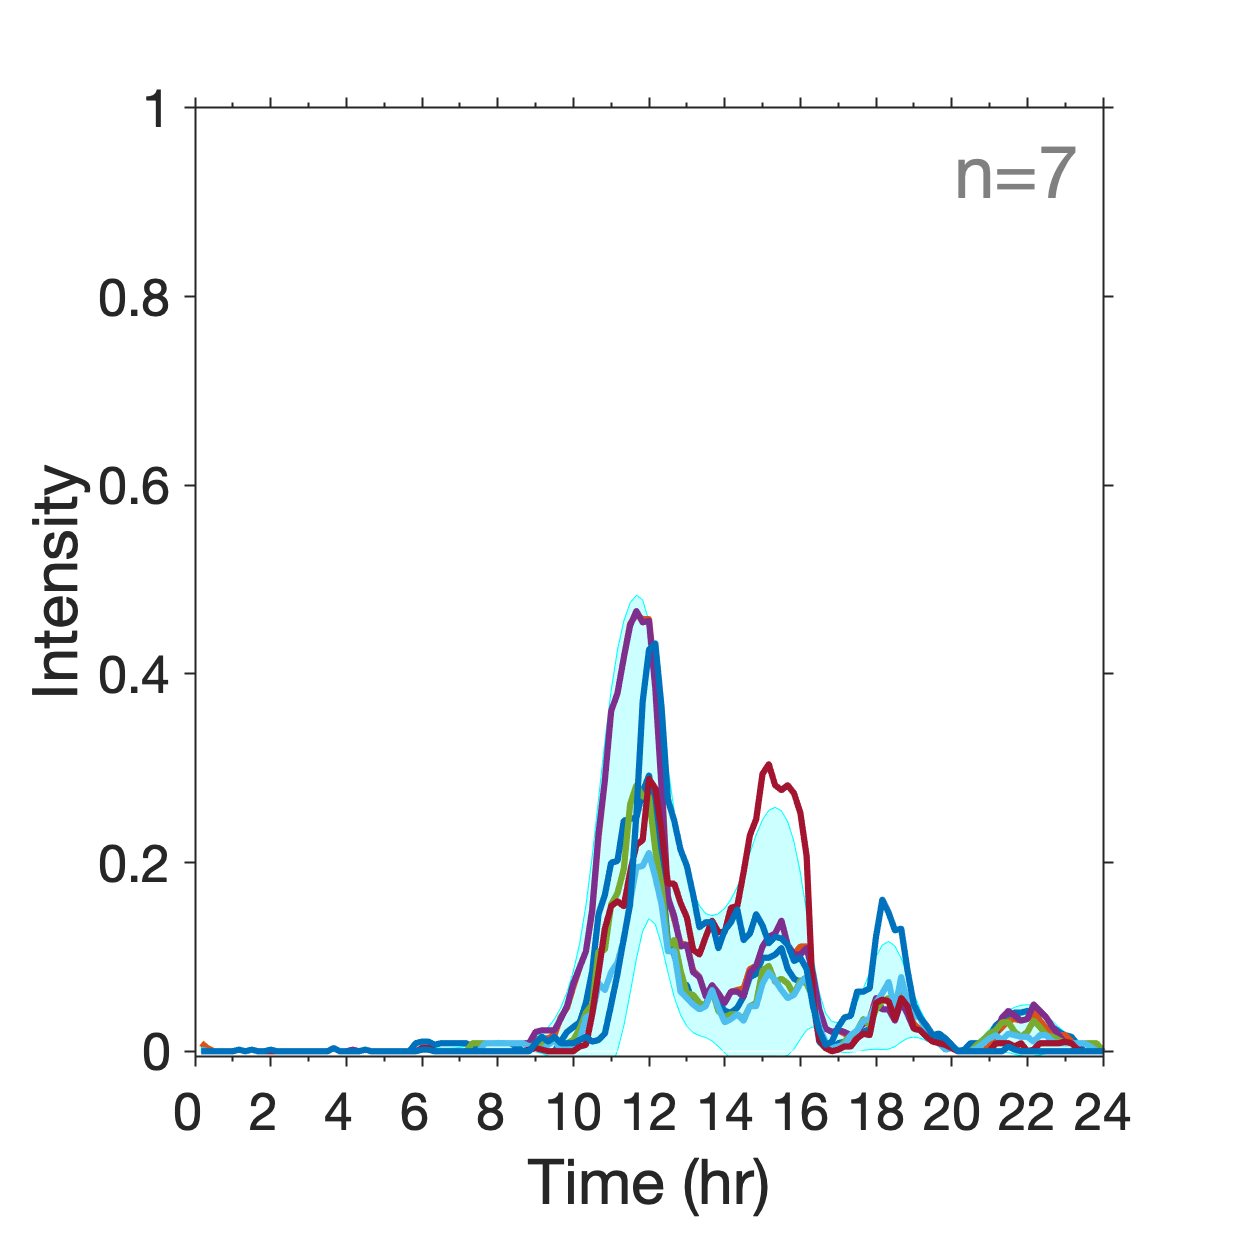
\includegraphics[scale=0.1]{../2Fittedy/plot/holiday_5/fitted_y_cluster5_4.eps} \\
			
			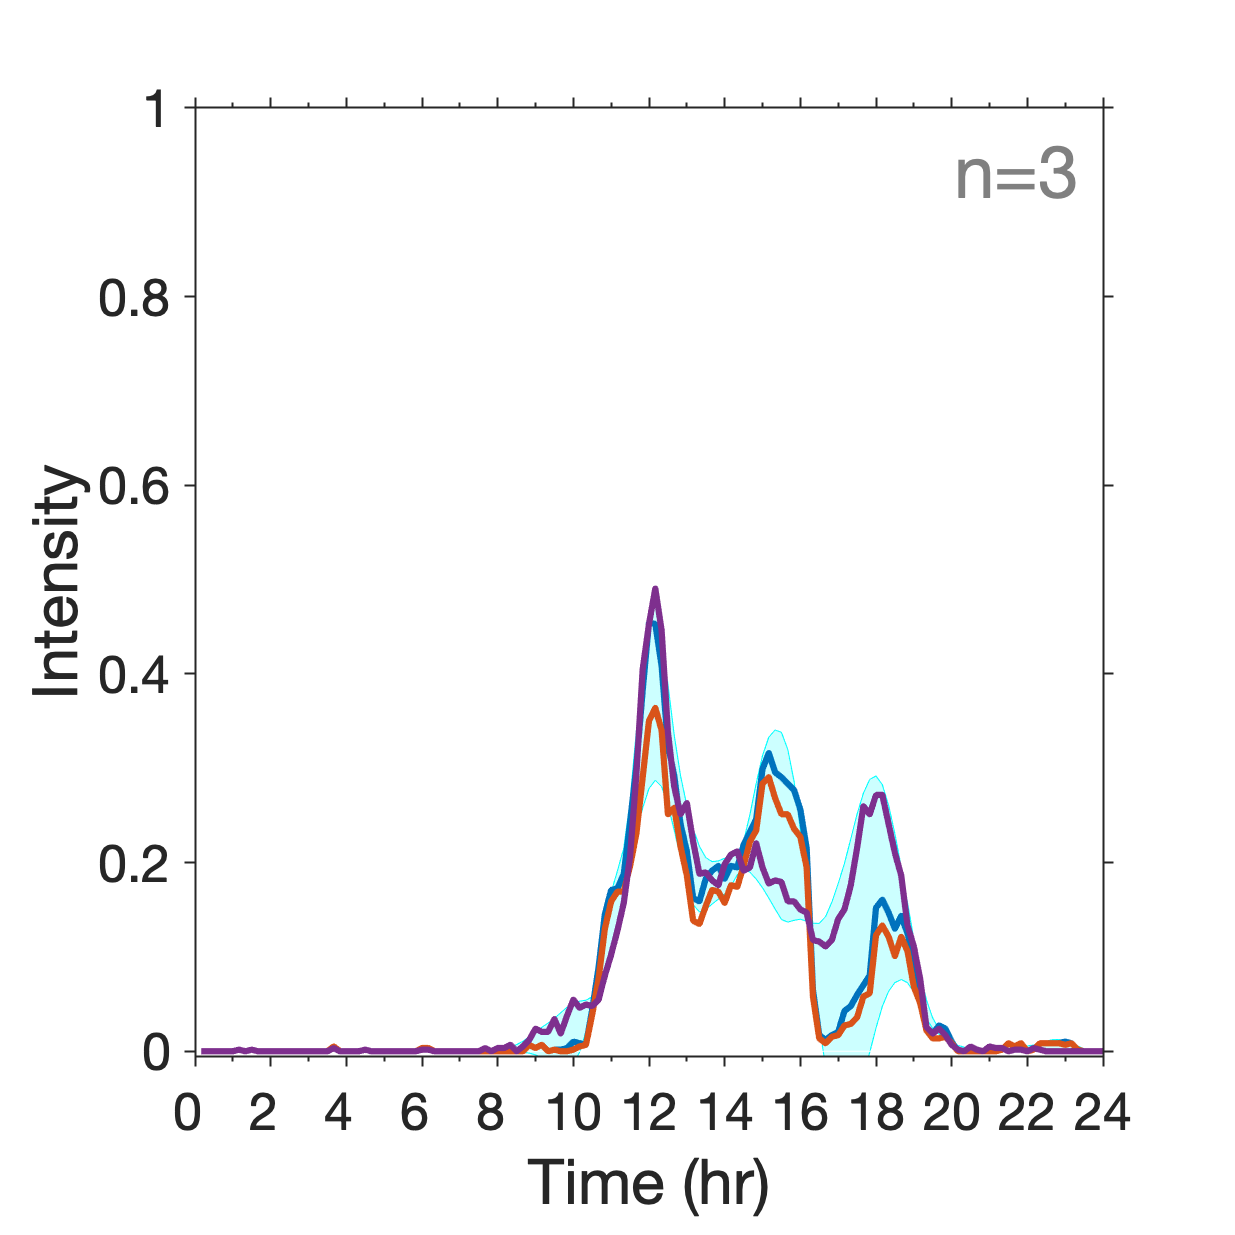
\includegraphics[scale=0.1]{../2Fittedy/plot/holiday_5/fitted_y_cluster5_5.eps} 
			&\hspace*{-0.6cm}
			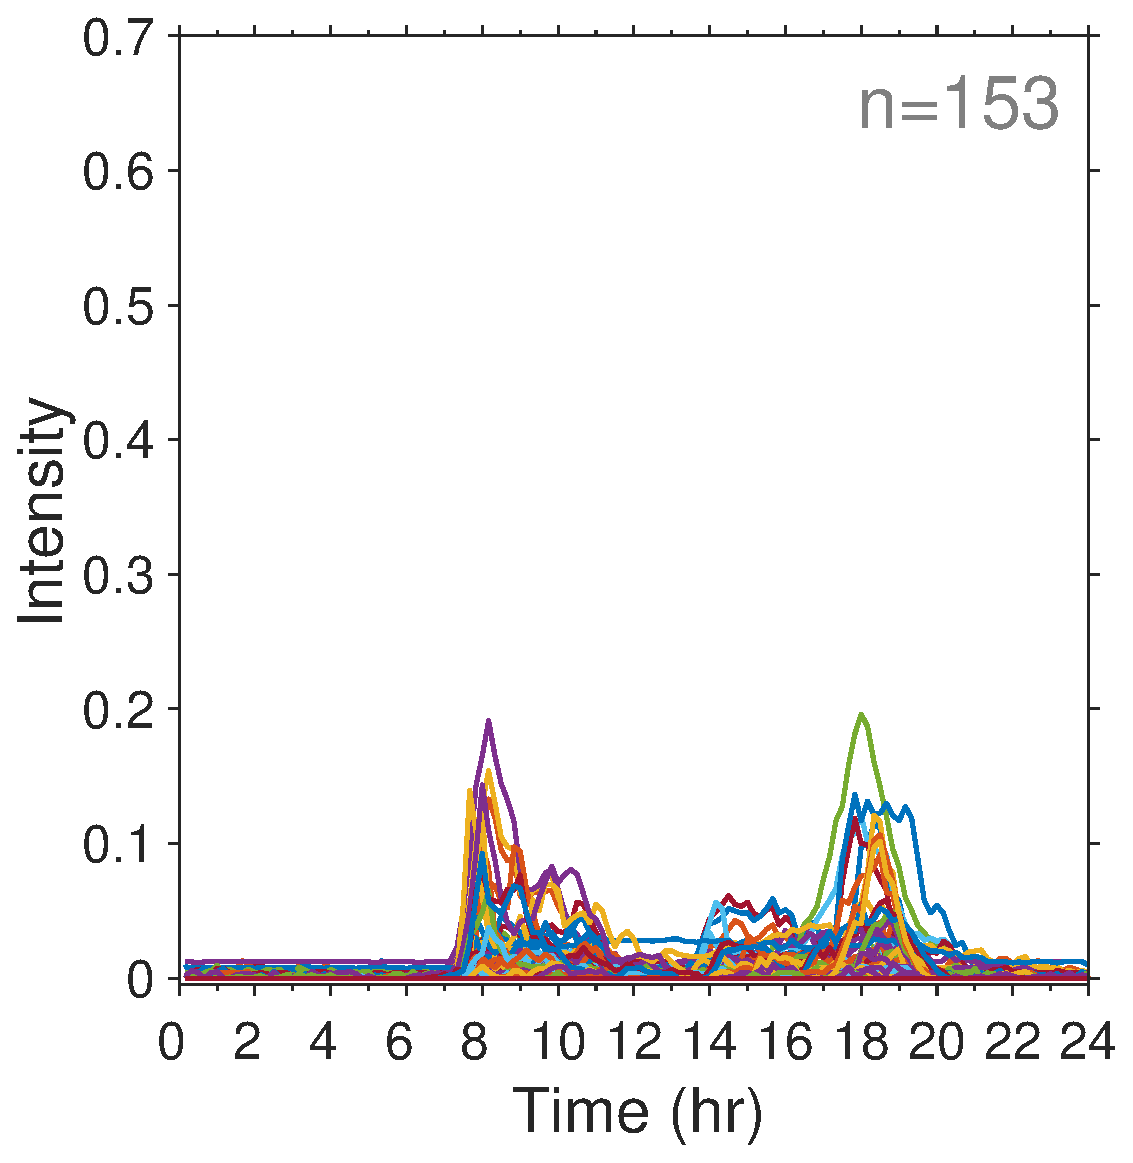
\includegraphics[scale=0.1]{../2Fittedy/plot/weekday_7/remove_data.eps} 
			&\hspace*{-0.6cm}

			&\hspace*{-0.6cm}

		\end{tabular}
		
		
		\caption{Holidays ($K_2=5$)}
	\end{center}
	
\end{figure}





\section{3Heatmap}
\begin{itemize}
	\item The file Heatmap.m in this file is the code that plots the heapmap.
	\item The input data are: detail\_weekday\_7.mat ($K_1=7$) and	detail\_holiday\_5.mat ($K_2=5$).
	\item And there are 2 output plots: one for the weekday group and one for the holiday group.
\end{itemize}
\begin{figure}[h!]
	\begin{center}
		\vspace{-0.3in}
		\subfloat[heatmap\_gray\_grid\_detail\_weekdayday\_5.eps]{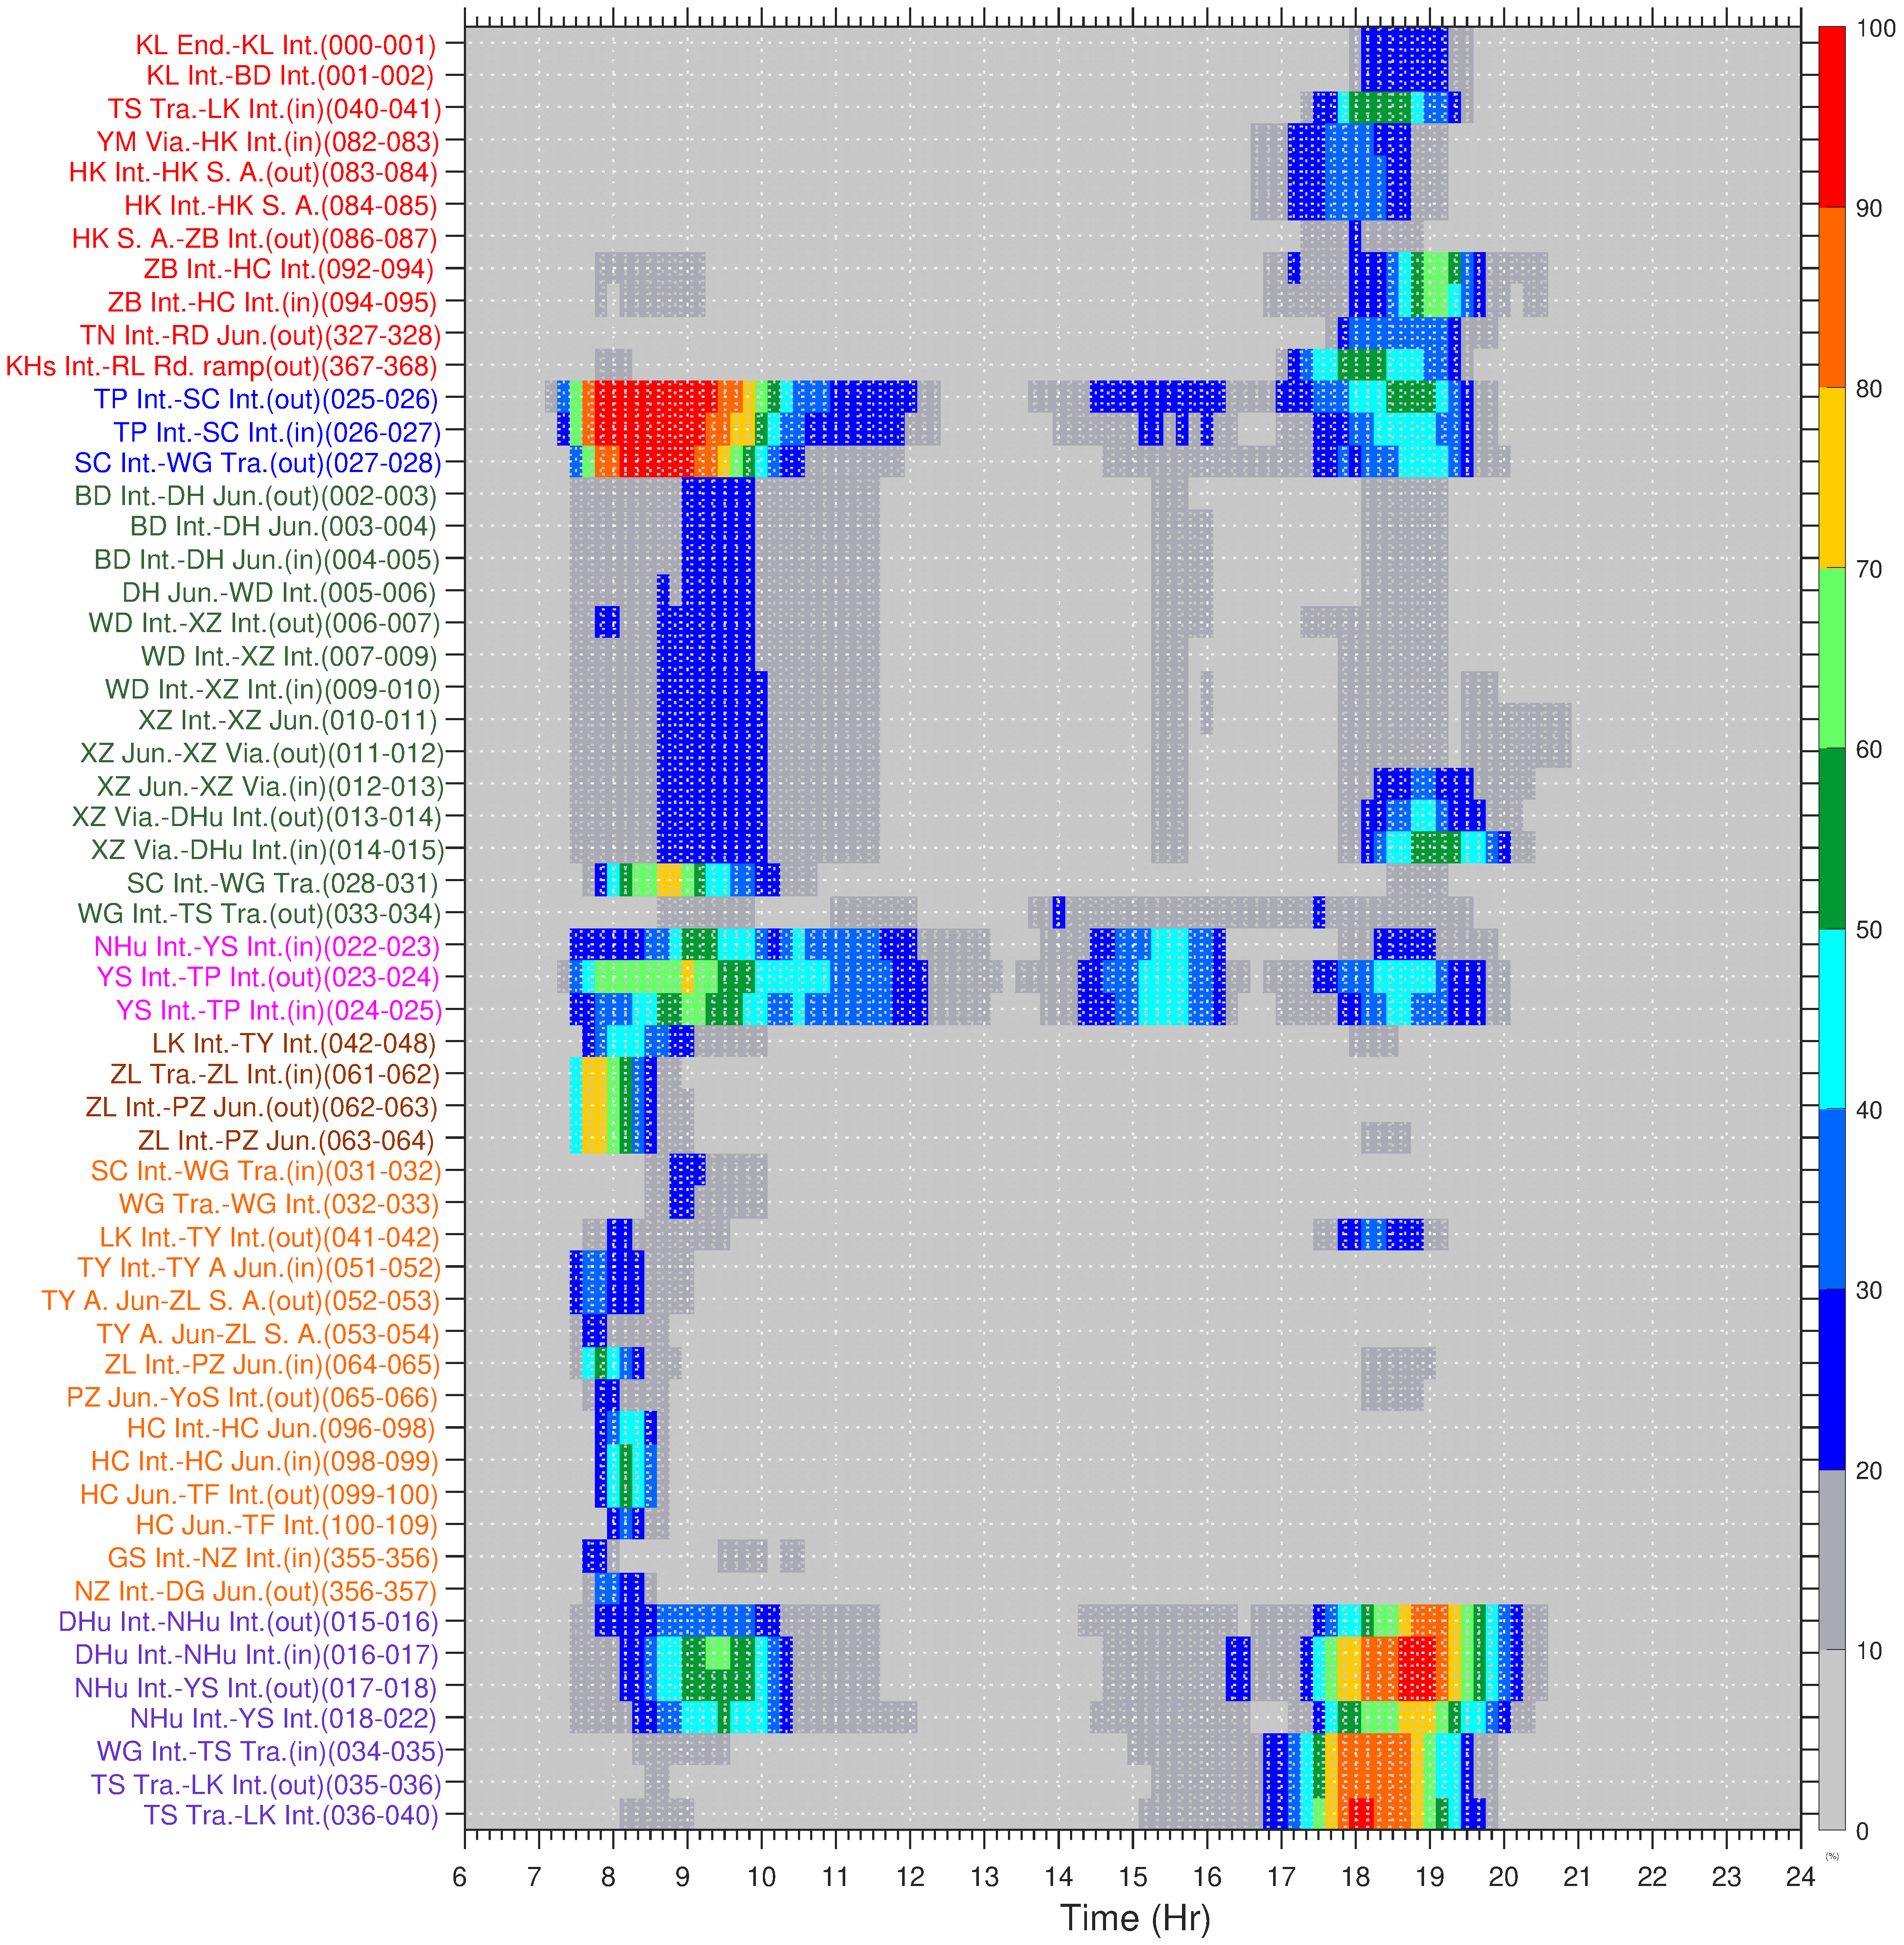
\includegraphics[width=7cm]{../3Heatmap/plot/heatmap_gray_grid_detail_weekday_7.eps}} 
		\subfloat[heatmap\_gray\_grid\_detail\_holiday\_5.eps]{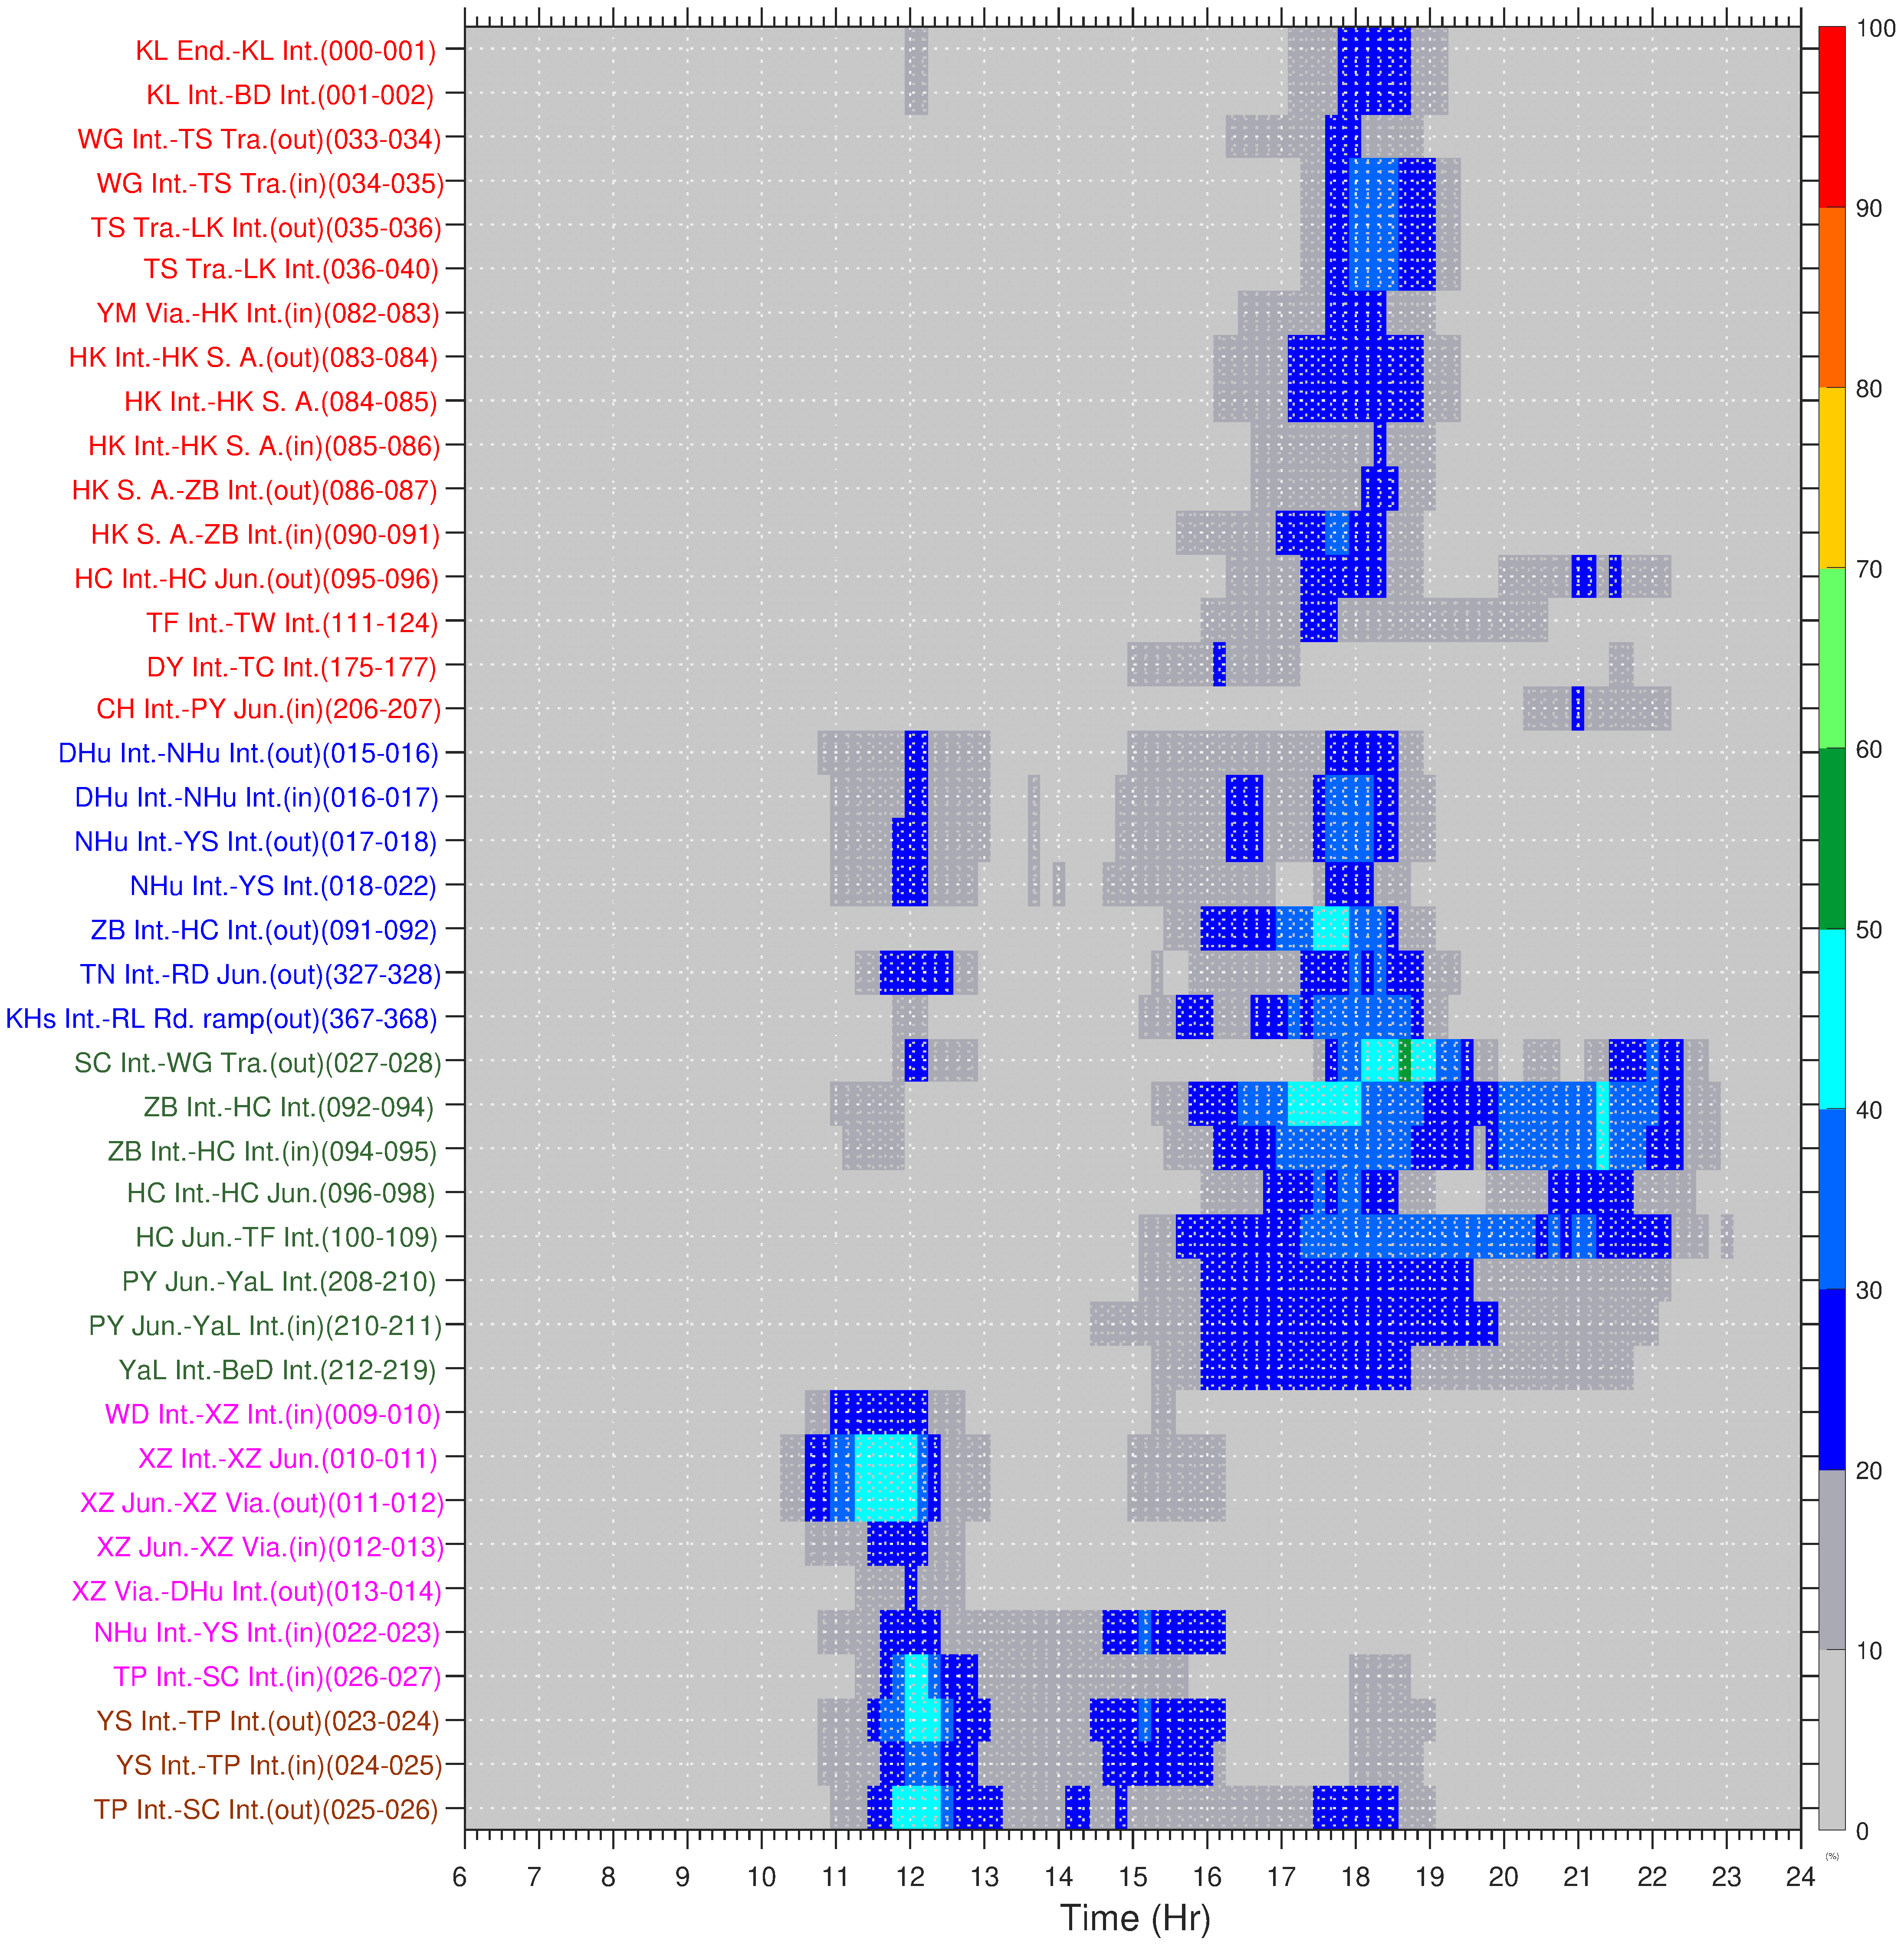
\includegraphics[width=7cm]{../3Heatmap/plot/heatmap_gray_grid_detail_holiday_5.eps}} 
		\caption{Hearmap}%
	\end{center}
\end{figure}



\section{4LocationCluster}
\begin{itemize}
	\item The file LocationCluster.m in this file is the code that plots the LocationCluster.
	\item The input data are: detail\_weekday\_7.mat ($K_1=7$) and	detail\_holiday\_5.mat ($K_2=5$).
	\item And there are 2 output plots: one for the weekday group and one for the holiday group.
\end{itemize}
\begin{figure}[h!]
	
	\begin{center}
		\vspace{-0.3in}
		\subfloat[weekday\_7.png]{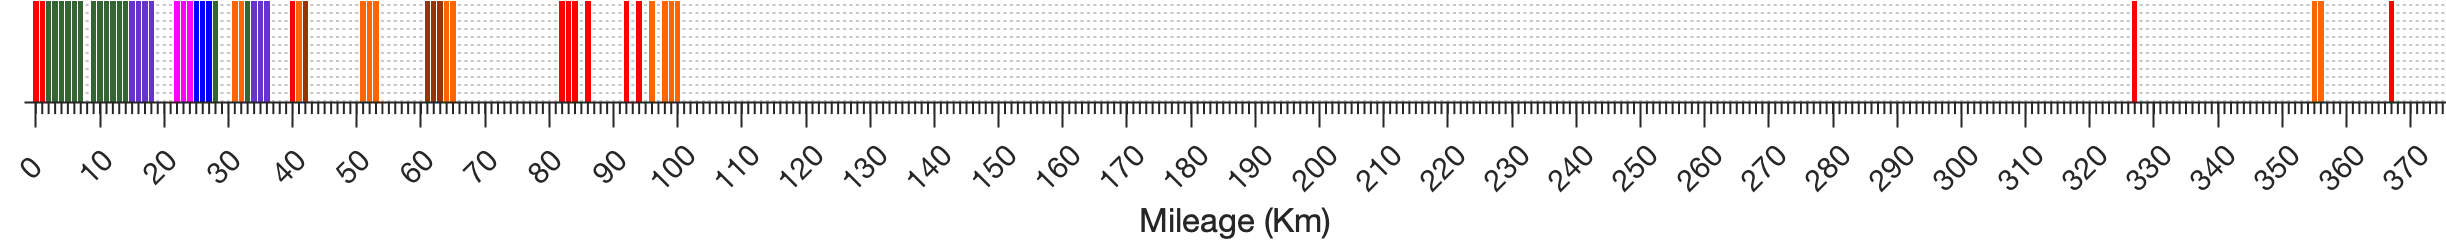
\includegraphics[width=7cm]{../4LocationCluster/plot/weekday_7.png}} 
		\subfloat[holiday\_5.png]{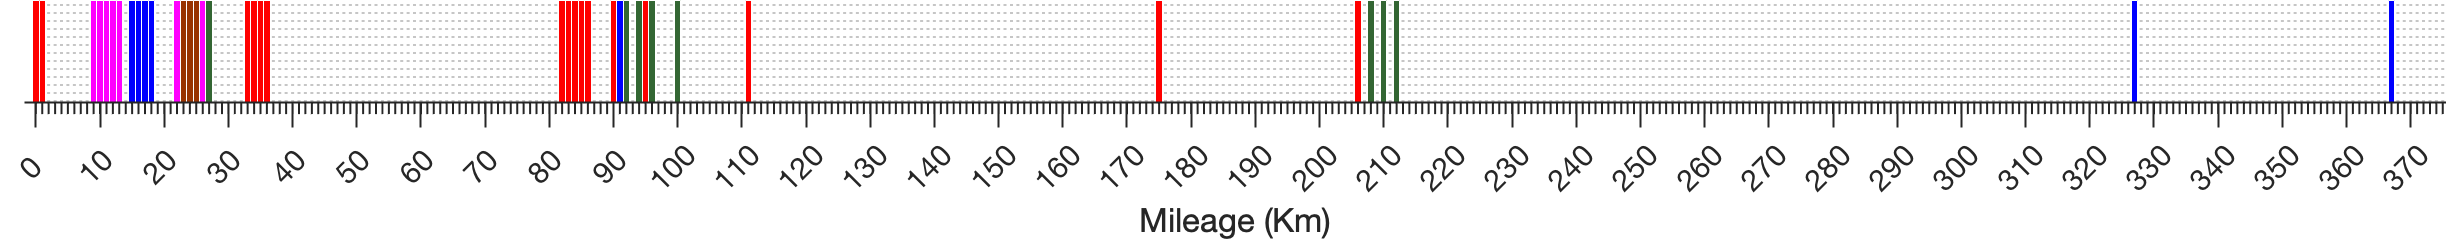
\includegraphics[width=7cm]{../4LocationCluster/plot/holiday_5.png}} 
		\caption{Point Process Diagram}%
	\end{center}
\end{figure}

\section{234Combine}
\begin{itemize}
	\item Since Fittedy.m, heatmap.m, and LocationCluster.m actually use the same input data of detail\_weekday\_7.mat ($K_1=7$) and	detail\_holiday\_5.mat ($K_2=5$).
	\item The file Combine.m can run them all together.
	\item I store the output in the folder plot. 
	\item In the folder plot, there are two files: weekday\_7 and holiday\_5.
	\item The folder weekday\_7 stores all the results of the weekday group.
		\item And the folder holiday\_5 stores all the results of the holiday group.
	

\end{itemize}
\end{document}